\documentclass[12pt]{article}
\usepackage{geometry}                % See geometry.pdf to learn the layout options. There are lots.
\geometry{letterpaper}                   % ... or a4paper or a5paper or ... 
%\geometry{landscape}                % Activate for for rotated page geometry
\usepackage{graphicx}
\usepackage{amssymb}
\usepackage{natbib}
\usepackage{subcaption}
\usepackage{longtable}
\usepackage{amsmath,amsthm,amsfonts}
\usepackage[dvipsnames]{xcolor}
\usepackage{colortbl}
\usepackage[colorlinks=true, pdfstartview=FitV, linkcolor=blue, 
            citecolor=blue, urlcolor=blue]{hyperref}

\usepackage[parfill]{parskip} 

\renewcommand{\refname}{Bibliography}
            
%\DeclareGraphicsRule{.tif}{png}{.png}{`convert #1 `dirname #1`/`basename #1 .tif`.png}

\title{Investigating Bayesian Networks For Reasoning with Evidence by Using Agent-Based Simulations}
\author{Ludi van Leeuwen   {\small (S3092836)} \\ [1cm]{\small Supervisor: Prof. dr. H.B. Verheij} \\  {\small Second reader: Prof. dr. L.C. Verbrugge}}
\date{\today}                                           % Activate to display a given date or no date






\begin{document}
\maketitle
\newpage

\section*{Abstract}
We can use Bayesian Networks for modelling criminal cases. However, there are many open questions about the use of Bayesian Networks in modelling these cases. A pertinent issue is the problem of evaluating these networks. The existing methods for evaluating Bayesian Networks on full court cases are not sufficient: there is not enough data to calculate accuracy, sensitivity analysis does not tell you if an outcome is wrong, testing on cumulative evidence is usually done for only one set of evidence. However, when we define a BN, we need the BN to be true over all possible evidence states. A systematic way of evaluating the response of a BN on all possible valuations of cumulative evidence is proposed in this paper, and illustrated by means of an agent-based simulation of a robbery. We create automatically generated BNs, and a manual BN with subjective probability estimates based on this simulation. We can evaluate both the automated and the manual network over all evidence states, these networks generally perform well. We also apply the method to a BN idiom, where we find that the evaluation method shows us a case where this idiom behaves unexpectedly. However, we also apply this method of evaluation to a BN that models a crime scenario without simulation. Here we find that the evaluation method is not generalisable due to combinatorial explosion of possible evidence states, the subjectivity in establishing a ground truth without using simulations, and the imprecision in node definitions in the BN.

\newpage

\tableofcontents
\newpage

\section{Introduction}
When we find evidence for a hypothesis that we have held in the back of our minds, our belief in that hypothesis increases. This is the essence of reasoning with evidence. Our goal in reasoning with evidence is to find a method that will lead us to believe the most relevant true hypothesis, given the evidence that we have.

However, the relationship between evidence and hypotheses is elusive. How can we be sure that a piece of evidence supports some hypothesis? Even if we know that it does, how can we express how strong the piece of evidence is? Some evidence is very weak, and only after a tedious process of ruling out other factors and careful investigation and collection of other pieces of evidence, we can come to a conclusion about a hypothesis. On the other hand, some evidence is so strong that it leaves no room for doubt.

We can consider three main approaches for reasoning about hypotheses using evidence within the domain of AI and Law \citep{diBelloVerheij2018}: an argumentative, a scenario-based, and a probabilistic approach. The argumentative approach models attack and defence relations between different arguments as supported by evidence. The scenario approach models conflicting coherent stories about the evidence. The probabilistic approach models evidence strength, how we should change our belief in a hypothesis once we learn some evidence about it \citep{diBelloVerheij2018}.  One subfield of the probabilistic approach is the use of Bayesian Networks. Bayesian Networks can make explicit, and set a normative standard for how our beliefs about events should change given that we find certain pieces of evidence for them. This should increase transparency and fairness in a courtroom. In the ideal case, a Bayesian Network might stop a judge from making a reasoning error.

However, creating and using BNs is far from straightforward for both the builder and the interpreter. From \citet{deKoeijer2020}: it is complex, time-consuming, hard to explain, and, the ``repeatability [...] leaves much to be desired. Node definitions and model structures are often directed by personal habits, resulting in different models for the same problem, depending on the expert''. This subjectivity is pervasive throughout the Bayesian Network: the events selected, arcs drawn, and numbers elicited are subjective and seem empirically untestable in the data-poor environment of AI and law. These problems might be mitigated in part by evaluation criteria. 

These evaluation criteria, however, do not always sufficiently safeguard against an incorrect network, which is a network that predicts the `wrong' outcome based on some set of evidence. A BN for crimes should be accurate across all possible evidence states, since, if we want to use BNs in court and not model court cases afterwards, we do not know at the start what the state of the evidence will be. However, in general, it is hard for modellers to rationally consider all possible evidence states. A network might respond well to situations where all evidence as presented in the trial is present, but predict the wrong outcome when one evidence node is turned to a different value. This brings up questions about the use of BNs in general: do we really need to consider these states where the evidence is different from the evidence as presented in the trial? Since specifying the joint probability distribution is necessary in BNs, we have to specify all of these numbers. 

The aim of this project is to define a method for the modeller to evaluate the BN over all possible evidence states, by grounding the BN in an agent-simulation of a crime. We can model crime cases using simulations to a level of realism we desire, measure the frequencies of events that emerge out of this simulation by running the simulation multiple times. In the agent-based system, we have full control over and full knowledge of the world that we are reasoning about, therefore we can generate `known' frequencies for all events that occur (also called `grounding' frequencies). These grounding frequencies can be used to evaluate the BN. We can test whether our method of evaluating all possible evidence states works by comparing the predicted output of the BN with the frequency information about the output from the simulation. Additionally, we create a manual Bayesian Network of the scenario and evaluate it using the known frequencies to discuss whether it is plausible that a modeller could find the correct subjective probabilities. Additionally, we apply the method for evaluating BNs to two different Bayesian Networks (those presented in \citet{deZoete2019} and \citet{vanLeeuwen2019}.  We also discuss the use of simulations as a modelling primitive. 
 \footnote{The simulation can be interacted with at \url{https://shielded-journey-34533.herokuapp.com} \\ Code for this project can be found at \url{https://github.com/aludi/simulationTest}}. 
 

\newpage

\section{Background}

% reasoning with evidence
%Ook kort bespreken/benoemen: Di Bello and Verheij (2018) discuss how central analytic goals can be handled using each of the approaches.
We want to create grounded Bayesian Networks for reasoning with evidence. This can be done by creating a agent-based simulation, building BNs based on the events in this simulation, and testing the evaluation method on that BN. In this section, the relevant background is laid out on reasoning with evidence, Bayesian Networks, existing evaluation methods for BNs, and agent-based simulations.


\subsection{Reasoning with evidence}
We consider three main directions in the field of reasoning with evidence within law \citep{Verheij2015}, \citep{diBelloVerheij2018}. 

The first direction is via argumentation approaches, where hypotheses and evidence are represented as propositions that attack or support each other, as originating in \citep{wigmore1931} and in part unified by \citet{dung1995}, for a historical overview see \citep{benchcapon2019}. An example of argumentation research in AI and law is ASPIC+ \citep{prakkenEtal2013}. 

The second direction is via scenario approaches, where coherent hypotheses are combined into stories \citep{penningtonHastie1993}, \citep{wagenaarEtal1993}, which are supported with evidence. Different types of stories need different pieces of evidence to be considered `valid' or `anchored' stories, and the extent to which different stories are anchored in the evidence determines how we assess them. 

The third direction is via probabilistic approaches, where hypotheses and evidence are assigned probabilities and the relation between hypothesis and evidence is represented with conditional probability, either by applying Bayes' law directly \citep{dahlman2020}, or by using Bayesian Networks. Bayesian Networks can represent aspects of a criminal case or can attempt a scenario-like hybrid and represent the entire case. Examples of this are: modelling actual crime cases \citep{kadaneSchum1996}, \citep{Fenton2019},  cases from fiction \citep{Fenton2012} or fictionalised crime cases \citep{vanLeeuwen2019}. The BN can also represent specific (forensic) aspects of a case, like DNA or blood-spatter evidence, for methods see \citep{Meester2021}. Bayesian Networks can also integrate aspects of argumentation \citep{wieten2019}, \citep{timmer2017}, or of scenario-based construction \citep{vlek2016}.



\subsection{Bayesian Networks}

A Bayesian Network (BN) is a directed acyclic graph that represents the joint probability distribution over a set of events \citep{pearl1988b}. BNs consists of nodes, arcs and conditional probability tables. A node is a random variable that represents an events. An arc represent a conditional relationships between two events, linking two nodes together. The two nodes are the parent and the child node, the probabilities in the child node are conditioned on the value that the parent node takes.


 The specification of these conditional probabilities is done in the conditional probability tables (CPT) of each node. As described in \citep{russellNorvig2010}:


The combination of all nodes in the BN results in a full joint probability distribution over all nodes, which is 
\[P(x_1, ..., x_n)\]

We can decompose this using the product rule

\[P(x_1, ..., x_n) =  P(x_n|x_{n-1},... x_1) P(x_{n-1},...x_1)\]

We see that $P(x_{n-1},...x_1)$ is also a joint distribution over all nodes, except node $x_n$. Hence, we apply the product rule again:

\[P(x_1, ..., x_n) =  P(x_n|x_{n-1},... x_1) P(x_{n-1}| x_{n-2}...x_1) P(x_{n-2},...x_1)\]

Keep applying this until we're at

\[P(x_1, ..., x_n) =  P(x_n|x_{n-1},... x_1) P(x_{n-1}| x_{n-2}...x_1) ... P(x_2 | x_1)P(x_1)\]

which is equivalent to 

\[P(x_1, ..., x_n) =  \prod_{i=1}^n P(x_i | x_{i-1},..., x_1)\]

In Bayesian Networks, we should connect the arcs between nodes such that the probability of the child node only depends on the value of the parents, and is independent from every other node. This assumption of conditional independence between non-connected nodes means that:

\[ P(x_i | x_{i-1},..., x_1) = P(x_i | parents(x_i))\]

So, every node $x_i$ is only conditionally dependent on its parents. This means that we drastically reduce the complexity if we can produce a BN where all nodes have the fewest number of parents as possible.

\[P(x_1, ..., x_n) =  \prod_{i=1}^n P(x_i | parents(x_i))\]

For every node $x$, hence, we do not have to specify the entire joint probability distribution. Instead, we can fill out the CPT by only taking into account all combinations of parent-node values.

\[P(x_i | parents(x_i))\]


We show an example BN in Figure~\ref{exampleBN}. This is the basic form of the evidence idiom \citep{Fenton2012}: we have a cause as a parent node, and a consequence as a child node. In this context, we want to interpret the parent node as a `hypothesis', that we want to prove, but cannot observe directly. The child node is a piece of evidence that we can observe: it is either true, or false. Specifically instantiated, like in Figure~\ref{exampleBN}, we create a basic scenario: `suspect shot victim with gun' as the parent (hypothesis) node, and `bullet casings found on ground' as the child (evidence) node. We can use this network, with the probabilities as defined in the CPTs, to reason about the hypothesis given the evidence that we find.
 
In Figure~\ref{exampleBN}, the node `suspect shot victim with gun' is a hypothesis. Nodes with one or more incoming arcs are conditionally dependent on their parent node(s). In our example network, the node `bullet casings found on the ground' is conditionally dependent on its parent. The links between the nodes are links of conditional probability, and do not correspond to real-world causality, although they are sometimes interpreted as being causal \citep{Dawid2008}.

\begin{figure}[htbp]
\begin{center}
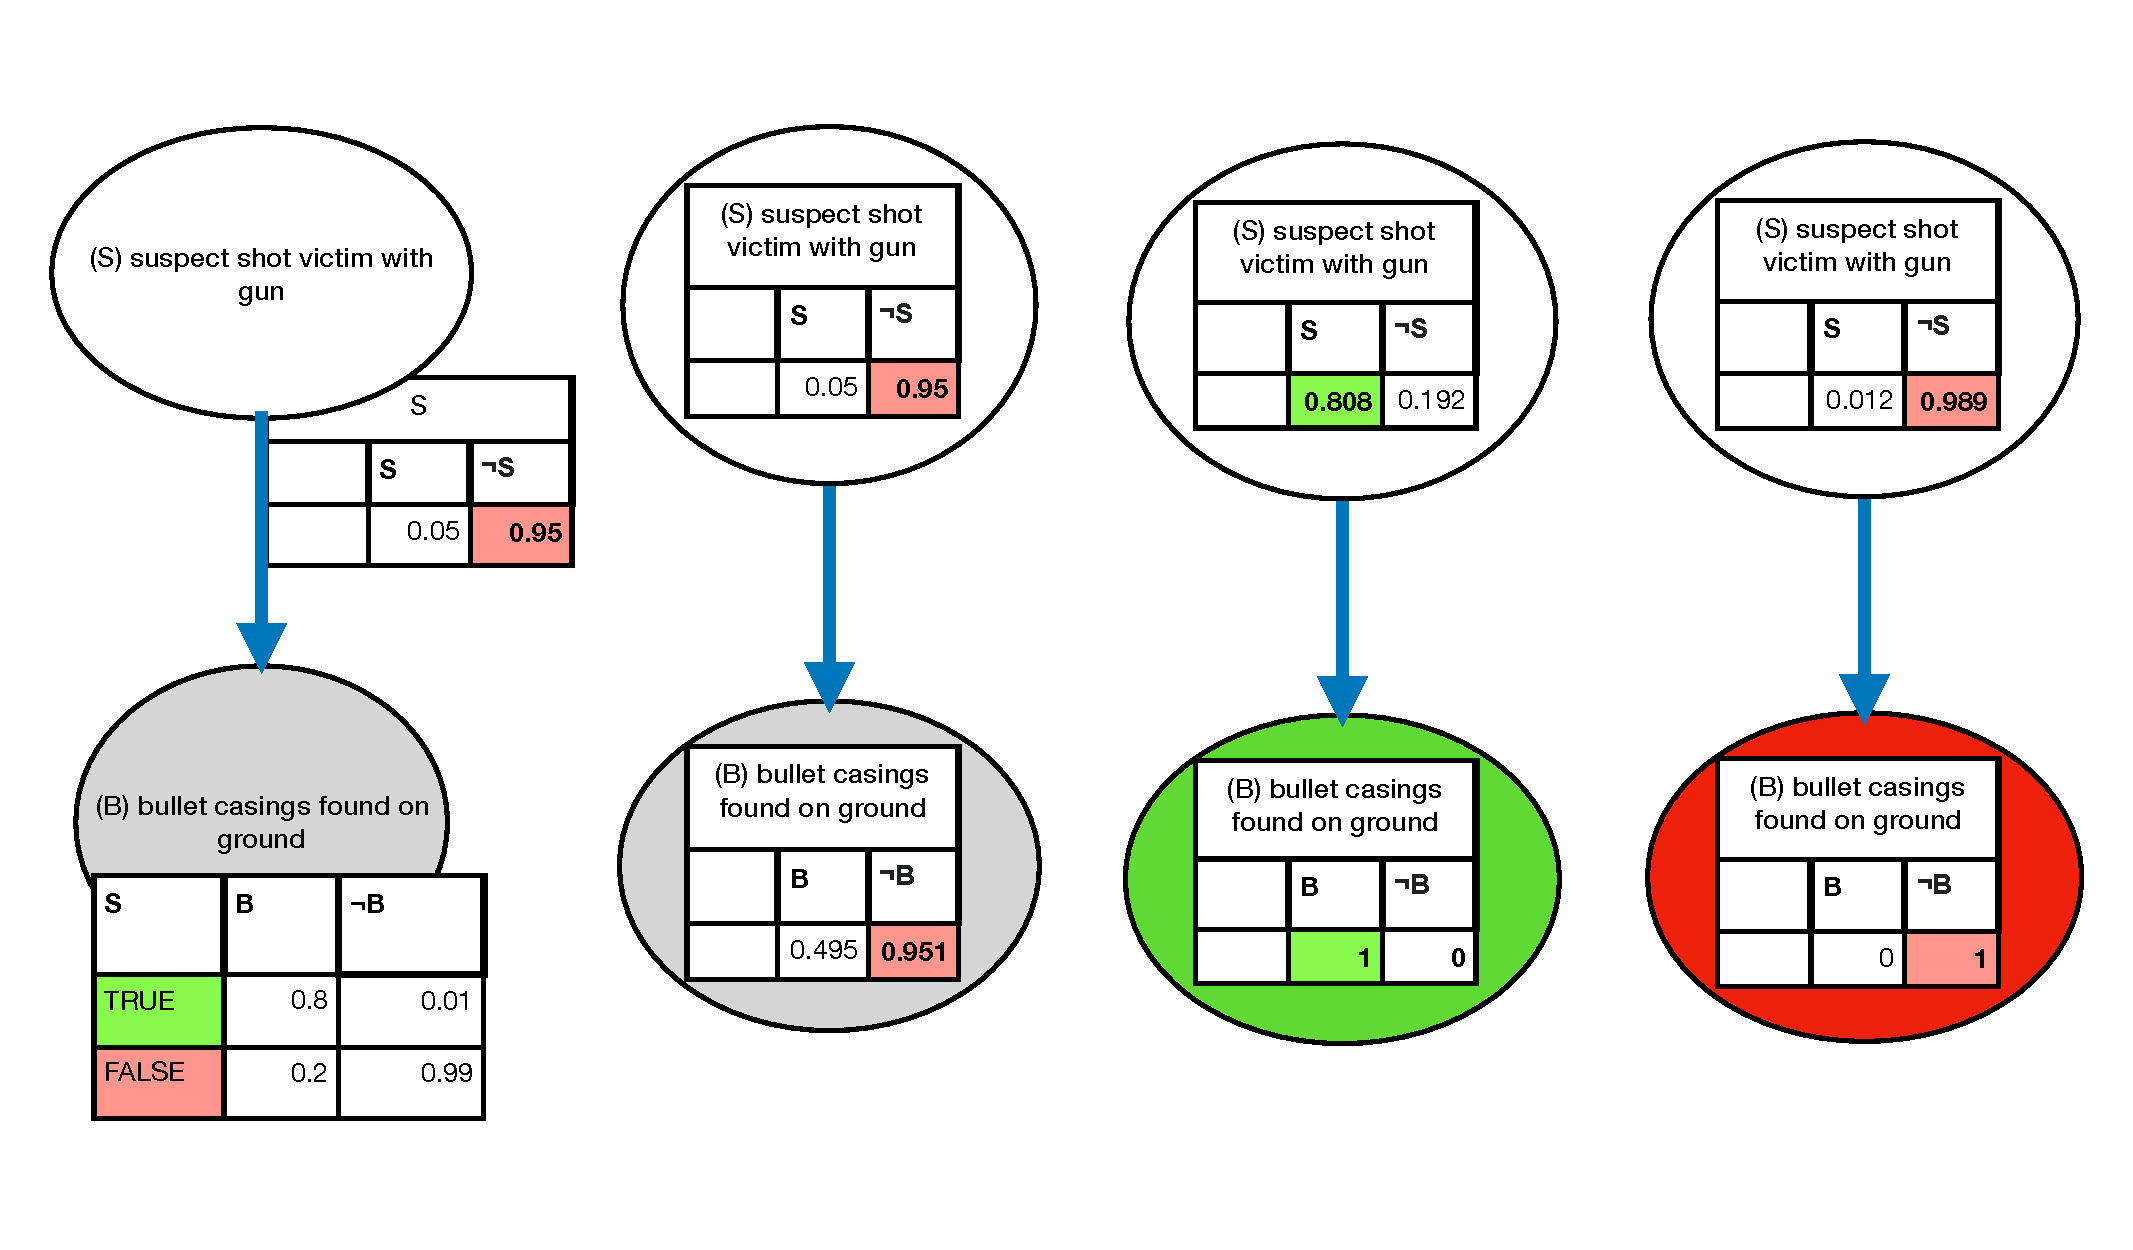
\includegraphics[width=\linewidth]{images/basicBayes}
\caption{Inference with Bayesian Networks: Defining the network with CPTS, entering no evidence, entering positive evidence, and entering negative evidence}
\label{exampleBN}
\end{center}
\end{figure}


The arcs and the CPTs tell us how we should reason about the hypothesis, given that we find some piece of evidence.


For a simple example, for a node with only one parent, we can just use Bayes law directly.


\[ P(H | E) =  \frac{P(E | H) \cdot P(H)}{P(E)}\]


To update to our network let us say that we found $B$, so there are bullet casings on the ground. We want to know what this new evidence will do to our belief in $S$. This means that we are updating our belief in $S$, or finding the posterior of $S$, based on the evidence that we found $B$.

\[ P(S | B) =  \frac{P(B | S) \cdot P(S)}{P(B)}\]
\[ P(B | S) = 0.8, P(S) = 0.05, P(B) = 0.8 \cdot 0.05 + 0.01 \cdot 0.95\]
\[ P(S | B) =  \frac{0.8 \cdot 0.05}{0.8 \cdot 0.05 + 0.01 \cdot 0.95} = 0.808\]

So now we have found the posterior of $S$, our belief in $S$ has increased from its prior probability of $0.05$, to its posterior probability of $0.808$, given evidence $B$. On the other hand, if we do not find bullet casings on the ground, our belief that the suspect shot the victim decreases from 00.5 to 0.012. 


Hence, we can exactly specify how our belief in a hypothetical event changes given all possible values of the evidence.This is the simplest form of Bayesian reasoning, with one piece of evidence, and one hypothesis. The general form of the update is more complicated and has high complexity (see \citep{russellNorvig2010} for an introduction to updating algorithms). We can use exact inference or approximate inference.


In real-life situations, we are constantly reasoning with many pieces of evidence that might be conditioned on more than one parent node, resulting in tedious and error-prone calculations if we would do them manually. This is where Bayesian Networks are useful. 



We can outsource the Bayesian calculation to the BN, however, the network itself has to be constructed in some way. This can be done by hand by modellers, or in (proprietary) software with a GUI like AgenaRisk or Hugin. They can also be built, by hand, or automatically constructed from datasets in PyAgrum, \citep{pyagrum2020}, a free Python software package. In this project, PyAgrum was used, using the LazyPropagation algorithm, which uses exact inference.



\subsubsection{Evaluating Bayesian Networks}

Bayesian Networks have been used to model reasoning with evidence in criminal cases, although these methods have not been used in court. However, even though there are methods for building BNs, it is unclear how we should validate and evaluate them. 

In data-rich domains, we can train Bayesian Networks on large amounts of frequency data and estimate the accuracy of the BN by cross-validation. We define a training set and a test set of the data (usually a 80/20 split). We construct the network based on the training data, 80\% of the input. Then, we test if the network learned the correct conditional probability relations on the final 20\% of the data, by comparing the expected output in the test data to the predicted output from the BN \citep{chen2012}. The 80/20 split allows us to measure to what extent the network is performing well on the entire dataset, and not just overfitting on the data that it has access to.

However, this approach towards BN validity through accuracy is implausible in BNs for court cases. The court cases involve one-of-a-kind events \citep{schum1982}, which means that it is unlikely that we can find frequency data on most of the nodes present in our BNs. This means that we cannot do an 80/20 type split in our data, as we only have one piece of data, which is the court case that we are modelling. This is why the probabilities in the BNs for court cases not pure frequencies, but instead subjective probabilities based on estimated frequencies, either elicited from experts or estimated by the modeller.

There are other ways of evaluating BNs than accuracy. The evaluation methods used by \citet{Fenton2019} and \citet{vlek2016}, who both model BNs based on real case studies, confine themselves to two approaches:

\begin{enumerate}

\item \textbf{Sensitivity analysis}

Sensitivity analysis tests which nodes have the greatest effect on a given target node. With sensitivity analysis, we can describe how much the target node will change if we make small changes in the conditional probability tables of those parent nodes \citep{fentonNeil2013}. This is useful if the outcome of the network hinges on elicited or subjectively estimated probabilities. In cases where we are eliciting data, or subjectively estimating it, it is often the case that we are in a data-poor environment, where using an accuracy measure as states above cannot be used due to extremely limited data. Hence, sensitivity analysis can be used to `sanity-check' elicited probabilities. If the target node is influenced by nodes that are unexpected given the causal relations that we are modelling, something has gone wrong. Since Bayesian Networks have many parameters per node, it is not trivial to perform a sensitivity analysis that takes into account all the nodes in the network and interpret the results in a meaningful way - this would be an $n$-way sensitivity analysis \citep{gaag2007}. We can also only define sensitivity analysis only for a given value of evidence: change the state of the evidence, and we might find different sensitivity values \citep{fentonNeil2013}. Various forms of sensitivity analysis are implemented in AgenaRisk and Hugin.

In \citet{vlek2016}, sensitivity analysis is mentioned, but not applied. On the other hand, in \citet{Fenton2019}, each individual hypothesis node is subjected to sensitivity analysis, to find out how every parameter in the nodes needs to change in order to result in a 0.95 or a 0.99 posterior for guilt. There are only a few ways that individual nodes can change that would result in a high probability of guilt, from which the authors interpret that the constructed BN is robust to small inaccuracies in subjectively elicited CPTs. However, in the paper, this is only shown for one evidence state. If the found pieces of evidence were to change, it is not clear if the BN would respond to this new evidence. 

\item \textbf{Cumulative evidence}

Another way of evaluating the response of the BN, is by seeing its response to cumulatively setting evidence. This way, we can see how much each piece of evidence (from the defence or the prosecution) changes our belief in the posterior of the output node(s). We could subjectively assess if it makes sense that a certain piece of evidence has a large, or small, effect on the posterior. In both \citep{Fenton2019} and \citep{vlek2016} this cumulative approach shows that, in general, the evidence from the defence decreases our belief that the suspect is guilty, and evidence from the prosecution increases our belief that the suspect is guilty. However, in both cases, the BN is only evaluated on one state of evidence. Both cases test the cumulative probability of the output node by turning the evidence nodes to values that correspond to the findings of the court and state the posteriors of the output nodes at every new evidence set, to see if the change in posterior corresponds to a reasonable evidence strength.



\end{enumerate}

However, these two existing methods do not ensure that a Bayesian Network correctly represents the criminal case across all possible values of evidence. Evaluating the network on just one evidence state is not sufficient. When we build a Bayesian Network, that network should perform well over all possible evidence states. This is important in court, where, if we build the model before the court case, we do not know the state of the evidence, hence, the evidence nodes could potentially take any value, and the network should predict the output correctly for any possible valuation. Additionally, even if we know the state of the evidence when we build the network, we could gain new information, like finding out that a testimony was not reliable after all, or that DNA was tampered with. In this case, we would want that information to propagate through the network correctly as well. Therefore, Bayesian Networks should not just be evaluated over one evidence state, but over all possible evidence states.


\subsection{Simulation}

We are using agent-based simulations to investigate methods for evaluating Bayesian Networks. Agent-based modelling is a modelling primitive that allows researchers to study models in which agents interact with their environment and with other agents \citep{gilbert2000}. 

In an agent-based simulation, we are essentially creating a mini-world in which we have total control over what can occur. We as modellers also are able to have full knowledge of what is happening within that world, since we have access to the total state space of the simulation. In these mini-worlds, `agents' abide by a set of behavioural rules that describe how they are able to interact with other agents and their environment. The `agent' metaphor allows us to reason about these computer-agents like we would reason about people in real life: the agents can walk, or run around, need to know certain things about other agents and can engage with these other agents (for example, by stealing from them). As we can create a spatially-explicit simulation, where agents `walk' around an environment, agents cannot move everywhere, and do not yet `know' anything. For instance, an agent cannot move through buildings like a ghost, or steal from someone they have not seen.

The way that we are programming the agents, can be as high-level or low-level as necessary, depending on the purpose of the simulation. We could create very realistic agents that walk around according to collected movement patterns from real people \citep{Zhu2021}, and implement complex sociological rules on criminal behaviour into the agents \citep{Gerritsen2015}. However, the agent rules do not have to be realistic or complex to create a simulation that is interesting as a grounding for a Bayesian Network. If we look at the taxonomy of agent-based model levels in \citep{gilbert2005}, where level 3 is a simulation that reflects the real world, and level 0 is a `caricature of reality, as established with simple graphical devices', the simulation in this paper is at level 0, to reduce unnecessary modelling and time complexity.

The purpose of the simulation in this paper is to model a criminal scenario. Due to specific interactions between agents that arise out of the circumstances in each run of the simulation, we can collect frequency information about all relevant events in our modelled scenario that would be hard to estimate with subjective probabilities or with mathematical (non-spatially explicit) models. Since we have full knowledge of the frequency of events in the simulation, we can use the simulation as a `grounding', or baseline. In a sense, the simulation is a data-generating environment for criminal cases.  In this project, the simulations are programmed in Python using the MESA framework  \citep{mesa2020}.

\newpage

\section{Method}

Our goal is to establish a method for evaluating BNs by preventing overfitting on one evidence state. We can consider an approach in four stages.

\begin{enumerate}
\item \emph{Scenarios} We need a set of alternative scenarios that are to be modelled. These scenarios are written description of crime scenarios that contain the hypothetical events and evidence for these events, as postulated by the prosecution and defence. 

\item  \emph{Simulation} Based on this written description of the scenario(s) to be modelled, an agent-based simulation is created, by first identifying and operationalising all relevant agents, objects and environments, and secondly identifying and operationalising all relevant events. Depending on the goal and complexity of the scenarios to be modelled, the granularity and overall level of the simulation should be considered. The simulation should be repeated until we find the limiting frequency of all events. These frequencies are collected.

\item  \emph{Construction} The collected frequencies are used by a construction algorithm to automatically build a Bayesian Network of the simulation. 

\item  \emph{Evaluation} The generated Bayesian Network is evaluated on all possible states of the evidence.

\end{enumerate}

\subsection{Scenarios}
We start our process with one or more written scenarios. These scenarios can be obtained from abridged or simplified court case descriptions of the crime, or they can be wholly fictional (such as in this paper). The scenarios should contain all and only those hypotheses and evidence that are relevant to the case. Both the prosecution and the defence should be able to select relevant events and their evidence. 

\subsection{Simulation}
We can think of the simulation as having two parts: a model of the scenarios, and a way of observing the model by observing variables that the modellers deem interesting. In this paper, the model of the scenarios is an agent-based simulation, and the observation procedure are random variables (or, reporters), which become nodes in the BN. Specifics about the model are explained in the next section.

\subsubsection{Model}

The agent-based simulation is a simulation that should include all events for all the scenarios as outlined in step 1. It should contain agents, objects and an environment. The agents should traverse the environment, interact with each other and using objects to be able to do certain interactions (think about stealing an object, or opening a door with a key).

The level of detail or real-world validation at which agents, objects and environments are modelled depend on the purposes of the simulation. In this paper, we are focussing on using simulations as a grounding to investigate Bayesian Networks. The detail of the simulation should be kept to the smallest complexity that is possible: it should be complex enough that Bayesian Networks can be usefully applied to it: there should be uncertainty, conditional probabilities, and different states. The focus should be on modelling nodes and only those nodes, that are relevant for the Bayesian Network method aspect that is under investigation: for example, creating a simulation to ground a network about the opportunity prior \citep{Fenton2017} or the scenario-idiom \citep{vlek2016}, or the abuse-idiom in ~\citet{deZoete2019}, as we do in this thesis. The simulation should not be made more complicated than necessary to limit debugging time and complexity.

\subsubsection{Reporters}

In the simulation, certain events can be brought about. Any of the events as specified in the model could occur. We need a way to observe these states: this is where reporters come in. A reporter is a random variable that reports the outcome of a relevant event in the simulation. The reporters are embedded in the code. If an event happens (or does not happen), the reporter reports that the event is true (or false). In essence, the reporter ($R$) is a random variable (RV). In short, a random variable is a function that maps an event ($e$) to a truth value:

\[ R : e \rightarrow \{0, 1\} \]
No matter how many reporters we define, we can combine all reporters at the end of one run of the simulation into a global state $G$.

\[ G = (e_0 \rightarrow \{0, 1\} \times e_1 \rightarrow \{0, 1\} \times ... \times e_n \rightarrow \{0, 1\})\]
 or, for $n$ reporters:
 
\[ G = R_1 \times R_2 \times... \times R_n\]

We collect these global states over the number of runs that we do for each experiment, which results in the output $O$ of this stage of the method, is a series of global states, one for each run:

\[ O = (G_0, G_1, ... G_{runs})\]

The output of this method is the collection of runs $O$, where each run is the global state $G$ of the simulation, as measured by the random variables $R$.

\subsection{Construction}
Every random variable $R$ defined as reporter, becomes a node in the Bayesian Network. We can now automatically generate the Bayesian Network, using an automated BN learner method as implemented in pyAgrum. There are several learners implemented in pyAgrum.\footnote{An introduction to structure learning using PyAgrum: \url{http://webia.lip6.fr/~phw/aGrUM/docs/last/notebooks/structuralLearning.ipynb.html}} The algorithm used in this experiment to structure the Bayesian Network from the simulation data is the K2 algorithm \citep{Cooper1992}. 

The K2 algorithm is a greedy search algorithm that attempts to maximise the posterior probability of the network by correctly connecting parent nodes to child nodes. It takes an ordering on the nodes as input. The first node in the ordering $X_0$ does not have any parents. For two nodes $X_i$ and $X_j$, $X_j$ cannot be the parent node of $X_i$ if $j > i$: a node can only have a parent that is earlier in the ordering. The algorithm processes each node $X_i$ by adding possible parent nodes to $X_i$ (as constrained by the ordering), and maximising the score of the network. The algorithm stops if there are no parents to add, no parents improve the score, or the node has reached the maximal number of parents \citep{Chen2008}.

Due to this ordering, the K2 algorithm is efficient. However, finding the ordering of the nodes as input for the network is not trivial.  A heuristic for finding an ordering on the nodes is that the ordering should reflect meaningful causal or temporal information present in the domain. 


\subsection{Evaluation}

We can evaluate the response of the Bayesian Network using the effect of cumulative evidence on the posterior probability of the output nodes. This means that we order the evidence nodes chronologically, then instantiate every evidence node to a truth value (either T or F) in order. Then, we measure the posterior probability of all output nodes, given the cumulative set of evidence. We do this for all evidence states, since we have to evaluate the network over all possible outputs. We propose a method for evaluating Bayesian Networks over all possible global evidence states in this paper. This method is described here.

\begin{enumerate}
\item \textbf{Run} Run the simulation to generate the `ground truth'. 
\item \textbf{BN} Select the BN we want to evaluate.
\item \textbf{Selection} From the BN, select all evidence nodes (a total of $e$) and the relevant outputs $O$.
\item \textbf{Order} Order the evidence nodes. The order can be chronological, or can be the order that the evidence was presented in a court case. Ordering is not necessary for the calculating the posterior on the cumulative evidence, but improves consistency for the modeller.
\item \textbf{Collect} Collect all evidence nodes, $e$ is the total number of evidence variables. This is the set of $2^e$ combinations of evidence. An evidence state is a valuation of evidence, where for every evidence node, a truth value is specified. 
\item \textbf{Subset} From the previous step, select only the possible evidence states. We can extract the possible evidence states automatically from a simulation: we run it many times, and select the states that occur at least once in the outcome. The possible evidence states can also be elicited from experts by asking them to manually consider each evidence state.
\item \textbf{Frequencies} For every possible evidence state, calculate the frequency distribution of the relevant outputs $O$ by finding the frequency at which every outcome occurs, for every evidence state. Speaking generically about two alternative, non-mutually exclusive outcomes scenario 1 (scn1) and scenario 2 (scn2), we need to find a probability distribution over $scn1, \neg scn1 \land scn2, \neg scn1 \land \neg scn2$ that is constrained by $P(scn1) + P(\neg scn1 \land scn2) + P(\neg scn1 \land \neg scn2) = 1$. Or, a weaker version, we create a preference ordering on $scn1, \neg scn1 \land scn2, \neg scn1 \land \neg scn2$, without specifying probabilities. 
We can automatically create the frequency distribution over outcomes for all states of evidence from the data gathered in the simulation. If we do not have access to frequency data, then subjective frequencies (or a preference ordering over the output) need to be elicited from experts.
\item \textbf{Posteriors} For every possible evidence state, turn the relevant nodes in the BN on in order. At each step, record the posterior probability over the outputs. Automatically convert the probability distribution over the outcomes into a preference ordering.
\item \textbf{Accuracy Evidence State} Compare the BN prediction of output nodes given evidence to the frequency distribution as established in step 5). Once all evidence is added, we can calculate the divergence of the BN prediction and the actual frequency given the cumulative evidence $E$ in the simulation by \[|P(output|E) - F(output|E)|\]
\item \textbf{Accuracy Total} Calculate the total accuracy per output node by \[\frac{\sum_{i=0}^{e}|P(output | E_i) - F(output| E_i)|}{e}\] For the preference ordering, we do the same, only we calculate a counting score: when the preference ordering extracted from the BN is the same as the one from the simulation, we give a point, otherwise we do not, then average this over all sets of evidence.
\end{enumerate}


\newpage


\section{Case Study: Robbery at Grote Markt}
We illustrate the method by means of applying it to a case study of a robbery at the Grote Markt, the central square in Groningen.

\subsection{Experimental Set-up}
BNs were created and evaluated based on different number of runs, to evaluate how the accuracy of the BN depends on the data available to it. 

We want to create both a ground truth, that are the frequencies that we're interested in, and then the probabilities that are going to approximate it so that we can check the accuracy of the network. To find the ground truth, we need to find the limiting frequencies of the events in the simulation, the simulation was run 10,000 times. One thing we want to find out is the necessity of precision on the outcome of the networks. This was done by changing the number of runs that the BN was created on. The different number of runs of the simulation were [1, 50, 100, 300, 500, 750, 1000~] for creating the BNs. One run of the simulation took 100 steps, or until both agents were in their target states. 


\subsection{Scenarios}


We have established three different scenarios. In all scenarios, there are two people walking around the Grote Markt. One person is young, and the other person is old and carries a valuable object. 

In scenario 1 (scn1), the young person sees the old person, assesses whether the object is valuable enough to risk stealing, and if the old person is vulnerable enough to steal from, and a motive is established. Then, if the young person has a motive, they will attempt to sneak up on the old person. When they get near, they steal from the old person.

In scenario 2 (scn2), the young person might still be doing all of the above (or they might not), however, before they can steal, or if they decide that they're not stealing at all, the old person drops the object accidentally.

In scenario 3, neither scenario 1 or scenario 2 happens. The people walk around at Grote Markt and then go home. We do not have to represent scenario 3 explicitly, it can be represented as neither scn1 nor scn2.

For our evidence, we have a psychological assessment of the young person, that assesses whether they are psychologically capable of stealing from the old person. We also have cameras at Grote Markt that show whether the young person was seen at all, or was seen stealing. Additionally, we have the fact that the object is gone or not.


%In our simulation, there are two agents walking around the area of Grote Markt. One of the agents is old and carries a valuable object. The other agent is young, and might potentially steal the object. There are three things that can happen in this simulation: nothing is stolen or lost, the object is lost accidentally by the old agent, or the object is stolen from the old agent by the potential thief. If the potential thief sees the potential victim, it decides whether the object is worth the risk of stealing, and if the potential victim is vulnerable enough to steal from. If both of these conditions are fulfilled, the agent becomes a potential thief, and now has a motive to steal from the old agent. The agent will attempt to sneak up on the victim, and steal the object from the old agent. At some point, the old agent realises that their valuable object is gone. As evidence, we have a psychological report that estimates whether the young agent is capable of the crime, we might have video footage of the thief stealing the object, and we have the fact that the potential thief shows up on camera. 

%Additionally, outside the described scenario, we also have access to the `mental' state of the potential thief, so we know whether they actually consider the old agent vulnerable, and whether they find the object itself valuable. We also know if the thief is actually intending to sneak up on the other agent.


\subsection{Simulation}		% REPLICABILITY

We need a way to transform the natural language descriptions of the events in the scenarios to observable events in the simulation. First, we identify all relevant actors, objects and environments in the scenario and operationalise them in a simulation. Second, we identify the relevant reporters. 



\subsubsection{Model} 


Agents can interact with other agents and with their environment. Every agent has features, functions and roles associated with them. The agents in this simulation are created from the MESA agent class. These are goal-based agents.
Based on the scenarios as described in the previous step, we want to create one older, vulnerable agent, and one younger potential thief. In principle, the simulation is flexible enough that any agent can be a thief, as motive is determined by a risk-trade-off and not something inherent to the agents themselves. However, since we wanted to avoid problems with identity and follow the scenarios, we made sure that only one agent would be the thief, by having it have an object that was not valuable and an age that was not vulnerable. The behaviour of the agents is depicted in Figure~\ref{behaviourGM}.



All agents have the following \textbf{attributes}:
\begin{description}
\item [role] Every agent has a role of either victim or thief. In a more realistic scenario this role would be assigned based on behaviour, but in this simulation, this was done at the start (because the scenario allows for one thief, and one victim). However, the role `thief' does not mean that the agent will actually steal, and the role `victim' does not mean that the agent will be robbed\footnote{From now on the `' around the roles are dropped}: if the victim drops the object, or if the thief and victim never meet, these roles are not fulfilled by the agents. Hence, the role only implies a certain potentiality.
\item [id] Every agent has an ID. The thief has ID 1, the victim has ID 0.
\item [object] The thief has an object with a value of 0, the victim's object has a value drawn from a uniform distribution between 500 and 1000. 
\item [goal location] The goal location of the agent is either it's initial goal location that was assigned at the start, or, when the agent has a motive, it is the current location of the victim agent. The initial goal location for each agent is drawn randomly from any of the accessible locations at the edge of the map.
\item [age] The thief's age was 25, the victimt's age was drawn from a uniform distribution between 60 and 90.
\item [risk threshold] The risk threshold for the victim agent was set to 5000, such that it is never worth for it to steal, the risk threshold for the thief is randomly drawn from a uniform distribution between 800 and 1200.
\item [age threshold] The age threshold signifies at what age an agent considers another agent vulnerable: older agents are more vulnerable than younger agents. The victim's age threshold is set to 100, it will only steal from agents that are 100 years or older. The thief's threshold is randomly drawn from a uniform distribution between 50 and 100.
\item [steal state] The possible steal states are described as follows:
	\begin{description}
	\item[N] Initial state and state that the agent returns to if they fail to perform the task assigned by their state
	\item [MOTIVE] Agent has selected a target (target is vulnerable and object is valuable)
	\item [SNEAK] Agent moves towards target's position
	\item[STEALING] Agent is near target and attempts to steal
	\item[SUCCESS] Agent has successfully stolen object
	\item[DONE] Agent has reached their goal location
	\item[LOSER] Agent has been stolen from
	\end{description}
\end{description}

All agents have the following \textbf{actions}:

\begin{description}
\item [hang around] Agents move around randomly.
\item [walk] Using standard mesa functionality, at every step of the agent, the agent moves 1 cell in the Moore neighborhood. The agent attempts to walk towards its goal state, whether that is a moving agent or their goal state. They move towards their goal state by taking the possible step that minimises the distance between their goal and themselves using the Euclidian distance as measure (this does not take buildings into account).
\item [escape]  Given the use of Euclidian distance instead of a smarter, geographically-informed approach (using waypoints or something similar), agents can get trapped in tight corners of the simulation when they're moving towards their goal. There is an epoch tracker that counts `stuckness' and then moves the agent into the `hang around' state, of random movement, for a given time. This means eventually the agent will randomly move away from the `stuckness'.
\item [see] every agent has a visual range of 10 cells. This means that all simulation objects (agents, objects) within that radius are selected. Actual vision is only calculated based on line-of-sight, which means that for each object in range, we use the Bresenham's line algorithm to select the relevant cell that lie on the `environment grid' in between the agent and the object that it is seeing. For every cell on the straight path between the two objects, we check whether it is `accessible' or `non-accessible'. Agents and light (vision), cannot pass through `non-accessible' cells. This is an abstraction, in real life there are windows. So if there's one `inaccessible' cell on the list of cells that are the straight line between seeing agent and object, the agent is not able to see the object. 
\item [decide valuable] Once the thief has a targeted victim, the thief knows the value of the object of the victim. In this function, the agent decides whether the object is worth stealing. If the value of the object is larger than the risk threshold of the agent, the object is deemed valuable.
\item [decide vulnerable] Once the thief has a targeted victim, the thief knows the age of the victim. In this function, the agent decides whether the victim is vulnerable enough to steal from: if the age of the victim is older than the age threshold, the thief considers the victim vulnerable.
\item [sneak] Agent moves to the position of the victim, only it can move with a radius of 2 (hence, at higher speed).
\item [steal] Whenever the thief is in the same cell as the victim - and they're both still within the simulation (so the victim has not reached its goal yet), the thief steals successfully.
\item [drop] Agent drops the object accidentally
\end{description}




The environment is a discrete grid of size $x=75$, $y = 50$ that represents the geography of the Grote Markt. The real area of interest is approximately 425m x 280m, as estimated by the distance tool on Google Maps. This means that one cell in the simulation is equivalent to a square of 5.6m x 5.6m in real life. An agent can move 1 cell per time-step, which means that, given an average human walking speed of 1.4m/s \footnote{\url{https://en.wikipedia.org/wiki/Preferred_walking_speed}}, one time-step is equivalent to 4 seconds in real life. For the purposes of this simulation, this spatial and time resolution is high enough.

To simulate which parts of the Grote Markt were accessible to the agents, we had to convert a map image of the Grote Markt into an agent-readable world. This was done by writing a method to convert screenshots of maps into an agent-readable environment. The map was screenshotted from \url{http://maps.stamen.com/terrain/#18/53.21618/6.57225} and converted into greyscale. A grid was overlaid on the image. On the greyscale map, the color of the buildings was in the range of (189, 199): cells within this range were coded as `inaccessible', since agents cannot walk through buildings. All other cells were `accessible'. This resulted in a map shared by all agents that constrained their movements. The map constrains both vision and movement of the agent: we used this map to calculate the sight lines of both cameras and agents. An agent or a camera can only see another agent if there are no `inaccessible' grid cell on the sight line between the two, and the other agent is within their visual range. The environment is shown in Figure~\ref{groteMarkt}.
 

 There are two types of objects in the simulations, which are the valuable object, and the cameras. 

 In the scenario, an object is described as being in the possession of agents, or lost accidentally. In this simulation, the object was operationalized as being a feature of the agent, and not as an individual thing by itself.
 
 There are 5 cameras in the simulation. They are placed randomly on the `accessible' cells on the map. Every camera has a visual radius of 5, corresponding to a range of 28m, which is about equivalent to the visual range of real-life security cameras~\footnote{\url{https://securitycamcenter.com/how-far-can-security-cameras-see/}}.
 


%\item \textbf{We select all relevant events from the written description and attempt to operationalise them in the simulation.}
\subsubsection{Reporters}
We divide all events of the simulation into three classes: either an event is `evidence' (E), a `hypothesis' (H), or an ultimate `outcome' (O). 
\begin{description}
\item[(H) motive\_1\_0 ] agent 1's steal state is MOTIVE.
\item[(H) sneak\_1\_0 ] agent 1's steal state is SNEAK.
\item[(O) stealing\_1\_0 ] agent 1's steal state is STEALING.
\item[(O) object\_dropped\_accidentally\_0 ] At every epoch, there is a 1/500 probability that the victim agent will drop the object by accident. If the object is dropped, this reporter is turned on.
\item[(E) E\_psych\_report\_1\_0 ] indicates a `psychological profile' for the thief, to establish whether they would be able to steal the object or not. If the thief does not have a motive, there is no chance that it is picked (in-simulation), hence no psych report is established, the reporter remains 0. If the thief has a motive, there is a 0.9 probability that the psych report indicated that the thief is capable of stealing, and 0.1 probability that the thief could not have stolen the object. In this second case, the psych report is incorrect. This reporter is not represented spatially in the simulation.
\item[(E) E\_camera\_1 ] agent 1 is seen on any one of the cameras.
\item[(E) E\_camera\_seen\_stealing\_1\_0 ]  if any camera sees agent 1 when agent 1's steal state is STEALING.
\item[(E) E\_object\_gone\_0 ] if the object is dropped accidentally, or if the object has been stolen.
\end{description}



A global state where the thief stole the object and all the evidence pointed in this direction, would be represented as (reporters in the same order as in the listing above):
 \[1,1,1,0,1,1,1,1,1\]



\begin{figure}[htbp]
\centering
\includegraphics[width=\linewidth]{images/behaviourAgents.pdf}
\caption{The behaviour of the agents. The nodes with rounded edges correspond to actions that only the thief can take.}
\label{behaviourGM}
\end{figure}

\begin{figure}[htbp]
\centering
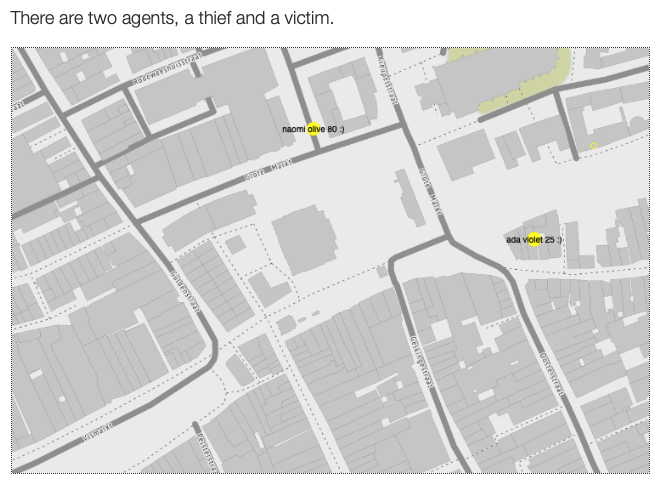
\includegraphics[width=0.75\linewidth]{images/grotemarktmap.png}
\caption{Map of environment. Dark grey represents roads, light grey and green represent open space, agents can traverse both. Mid-tone grey represents buildings, agents cannot move through them. Yellow circles are agents.}
\label{groteMarkt1}
\end{figure}

\begin{figure}[htbp]
\centering
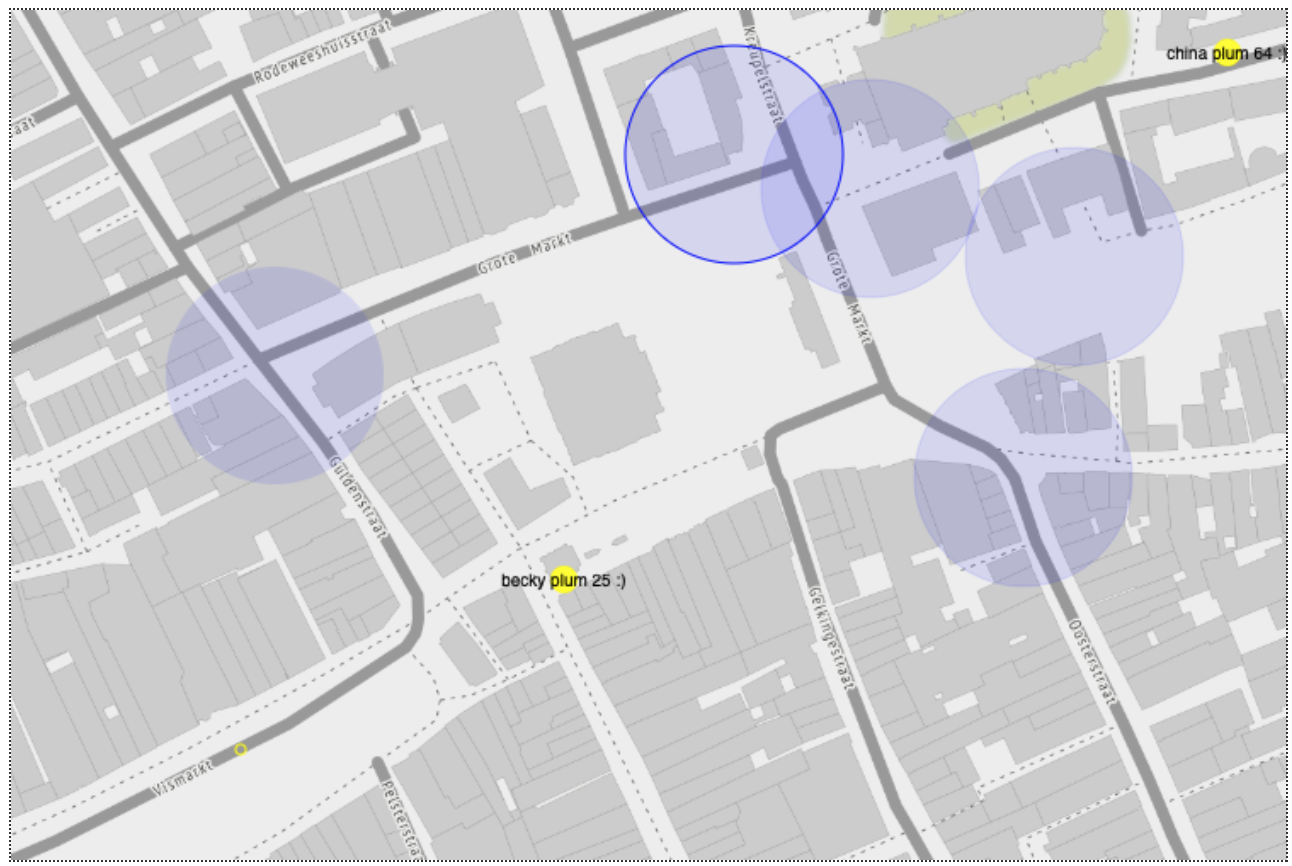
\includegraphics[width=0.75\linewidth]{images/agentGM.png}
\caption{Camera locations are randomly initialized. Blue circle represents the camera vision radius.}
\label{groteMarkt}
\end{figure}


\subsection{Construction}
To test to what extent the amount of data available to the K2 algorithm influences the accuracy of the network, for each of [1, 50, 100, 300, 500, 750, 1000~] runs, the collection of runs $O$ was passed to the K2 algorithm, which generates a network.

The K2 algorithm requires an ordering on the nodes. In all number of runs, this ordering was 
[object\_dropped\_accidentally\_0, motive\_1\_0, sneak\_1\_0, stealing\_1\_0, E\_psych report\_1\_0, E\_camera\_1, E\_camera\_seen\_stealing\_1\_0, E\_object\_gone\_0]. This ordering was determined by considering the hypothesis-nodes first, and all evidence at the end. We want evidence nodes to be the children of hypotheses nodes, to follow the hypothesis-evidence idiom as established by Fenton. This means that we have to add them the latest in the ordering, so that they will not be parent nodes to hypothesis nodes. The hypothesis nodes belong to two different scenarios: scenario 1 is the motive-sneak-steal scenario, and scenario 2 is the accidental-object-dropped scenario (scn2). Placing scn2 before scn1 in the ordering is not arbitrary. We have to invoke causality in order to establish that this is a sensible ordering: if the agent drops the object, the thief cannot have a motive to steal the object, yet, having a motive does not `cause' or `condition' the object to drop. Hence, the `object\_dropped\_accidentally\_0' should be the parent node, if we're taking a causal interpretation. We are not required to place scn2 before scn1 in the ordering if we are only using conditional probabilities as constraint.
 


\subsection{Evaluation}
\begin{enumerate}
\item \textbf{Run} We run the simulation 10,000 times to collect the ground truth.
\item \textbf{BN} We test all the BNs that we generated. We are generating 7 BNs, every one generated from a dataset with a different size:  [1, 50, 100, 300, 500, 750, 1000~]. This means we do this evaluation loop 7 times, each time testing a different BN.
\item \textbf{Selection} The evidence nodes of the network are the 4 (binary) nodes marked with an `E', which are [E\_camera\_1, E\_camera\_seen\_stealing\_1\_0, E\_object\_gone\_0, E\_psych\_report\_1\_0]. The output nodes are [`object\_dropped\_accidentally\_0', `stealing\_1\_0'].
\item \textbf{Order} We order the evidence nodes in the same order as they were presented to the K2 algorithm:  [E\_psych\_report\_1\_0, E\_camera\_1,  E\_camera\_seen\_stealing\_1\_0, E\_object\_gone\_0~].
\item \textbf{Collect} There are $2^4 = 16$ evidence states in total.
\item \textbf{Subset} We can eliminate $7$ of the evidence states, because they never occur in simulation. In Table~\ref{wake}, we present an overview of all possible states as generated by the and, if they do not occur at all, why they are impossible.
\begin{table}[htbp]
\begin{center}
\begin{tabular}{|l|l|}
\hline
state & remarks \\
\hline
(0, 0, 0, 0)  & ok\\
(0, 0, 0, 1) & ok\\
(0, 0, 1, 0) & we cannot have stealing on camera if the agent was not seen on camera\\
(0, 0, 1, 1) & we cannot have stealing on camera if the agent was not seen on camera\\
(0, 1, 0, 0) & ok\\
(0, 1, 0, 1) & ok \\
(0, 1, 1, 0) & we cannot have stealing on camera without the object being gone\\
(0, 1, 1, 1) & ok\\
(1, 0, 0, 0) & ok\\
(1, 0, 0, 1) & ok\\
(1, 0, 1, 0) & we cannot have stealing on camera without the object being gone\\
(1, 0, 1, 1) & we cannot have stealing on camera if the agent was not seen on camera\\
(1, 1, 0, 0) & we cannot have both psychological report, agent on camera, and not have stealing \\
(1, 1, 0, 1) & ok\\
(1, 1, 1, 0) & we cannot have stealing on camera without the object being gone\\
(1, 1, 1, 1) & ok\\
\hline
\end{tabular}
\end{center}
\caption{Possible and impossible states}
\label{wake}
\end{table}
\item \textbf{Frequencies} Using the possible evidence states identified in the previous step, in the ground truth dataset of 10,000 items, calculate the frequency distribution over the possible outcomes. In Table~\ref{heretic} we present the frequencies as generated by the ground truth of the three outcomes, as well as their preference ordering.
\begin{table}[htbp]
\begin{center}
\begin{tabular}{|l|c|c|c|}
\hline
evidence & H1 & H2 & H3 \\
\hline
(0, 0, 0, 1)&F(dropped) (0.99) & F(steal) (0.01) & F(neither) (0.00) \\
(0, 0, 0, 0)&F(neither) (1.00) & F(steal) (0.00) & F(dropped) (0.00) \\
(0, 1, 0, 1)&F(dropped) (0.99) & F(steal) (0.01) & F(neither) (0.00) \\
(1, 0, 0, 1)&F(steal) (0.93) & F(dropped) (0.07) & F(neither) (0.00) \\
(0, 1, 0, 0)&F(neither) (1.00) & F(steal) (0.00) & F(dropped) (0.00) \\
(1, 1, 0, 1)&F(steal) (0.93) & F(dropped) (0.07) & F(neither) (0.00) \\
(1, 1, 1, 1)&F(steal) (0.95) & F(dropped) (0.05) & F(neither) (0.00) \\
(1, 0, 0, 0)&F(neither) (1.00) & F(steal) (0.00) & F(dropped) (0.00) \\
(0, 1, 1, 1)&F(steal) (1.00) & F(dropped) (0.00) & F(neither) (0.00) \\
\hline
\end{tabular}
\end{center}
\caption{Frequencies of outcomes for all possible evidence states}
\label{heretic}
\end{table}

\item \textbf{Posteriors} For every evidence state, we use the BN as model. In the BN, we turn the evidence nodes to the value specified by their evidence state. We used the LazyPropagation inference engine in PyAgrum to calculate the posteriors of the outcomes in the BN, given the evidence state as input. 

\item \textbf{Accuracy Evidence State} The posteriors of the outcome nodes in the network are compared to frequency of those outcomes in the ground truth. The accuracy of the BN per evidence state is presented in the next section.
\item \textbf{Accuracy Total} The total accuracy per output node is presented in the next section. 
\end{enumerate}



\section{Results}


We have the final Bayesian Networks (Figure~\ref{bullet}) as created by the K2 algorithm to the runs from the simulation, except when we run the simulation 1 time. If we run the simulation 1 time, the network cannot be produced, as there is not enough data available to the algorithm. In Figure~\ref{bullet}, we can see that the structure of the network is not stable: the parents of the nodes depend on the number of runs that were available to the K2 algorithm.

However, despite the variability in network structure, all networks have some important commonalities. In all networks, we see that the evidence `E\_object\_gone\_0' has the parents `stealing\_1\_0' and `object\_dropped\_accidentally\_0', which correctly reflects the two events under which the object can be done. We also find that generally, `motive\_1\_0' is a parent node of `stealing\_1\_0', which reflects the underlying causality that the agent cannot steal without having a motive.
 
\begin{figure}[htbp]
\begin{center}
\begin{subfigure}{0.45\textwidth}
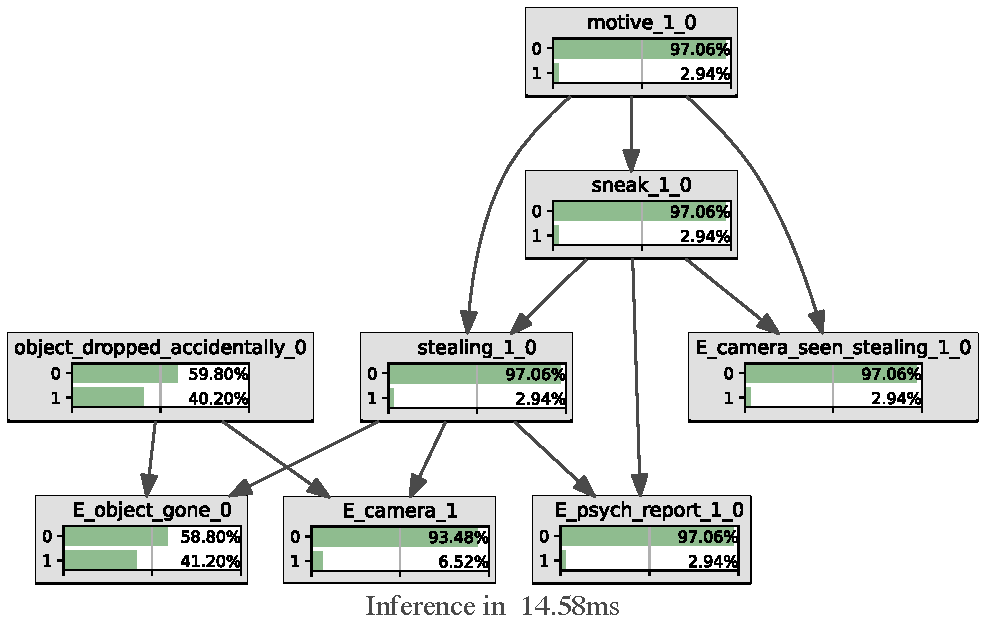
\includegraphics[width=\linewidth]{GroteMarktPrivate/bnImage/BNIMAGEGroteMarktPrivate50.pdf}
\caption{The final network (50 runs)}
\end{subfigure}
\begin{subfigure}{0.45\textwidth}
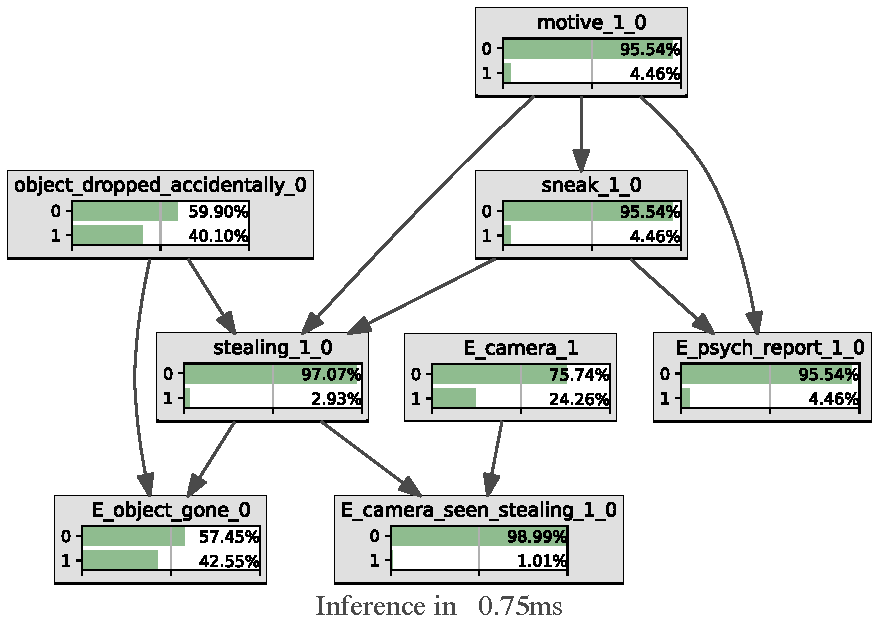
\includegraphics[width=\linewidth]{GroteMarktPrivate/bnImage/BNIMAGEGroteMarktPrivate100.pdf}
\caption{The final network (100 runs)}
\end{subfigure}
\begin{subfigure}{0.45\textwidth}
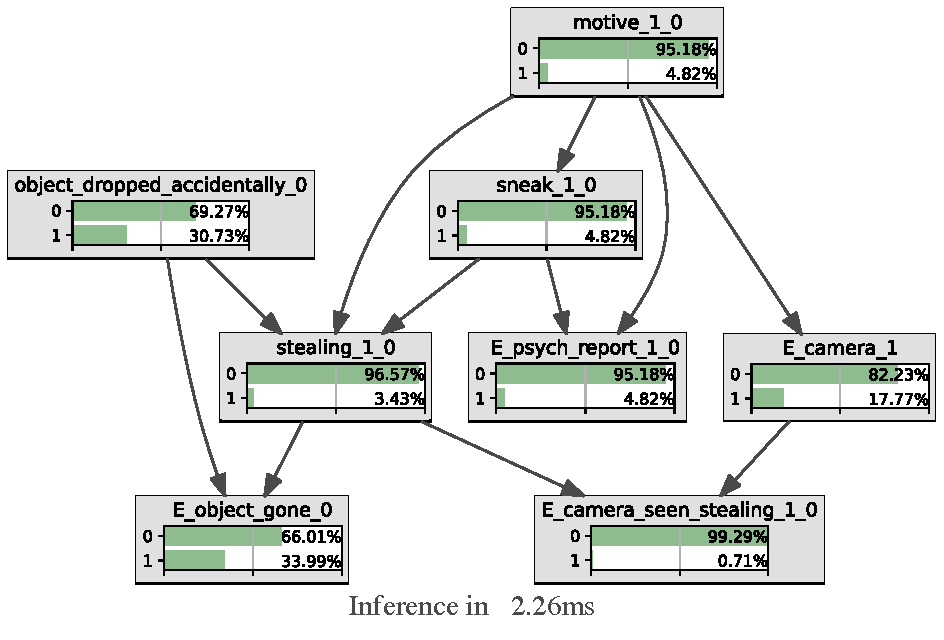
\includegraphics[width=\linewidth]{GroteMarktPrivate/bnImage/BNIMAGEGroteMarktPrivate300.pdf}
\caption{The final network (300 runs)}
\end{subfigure}
\begin{subfigure}{0.45\textwidth}
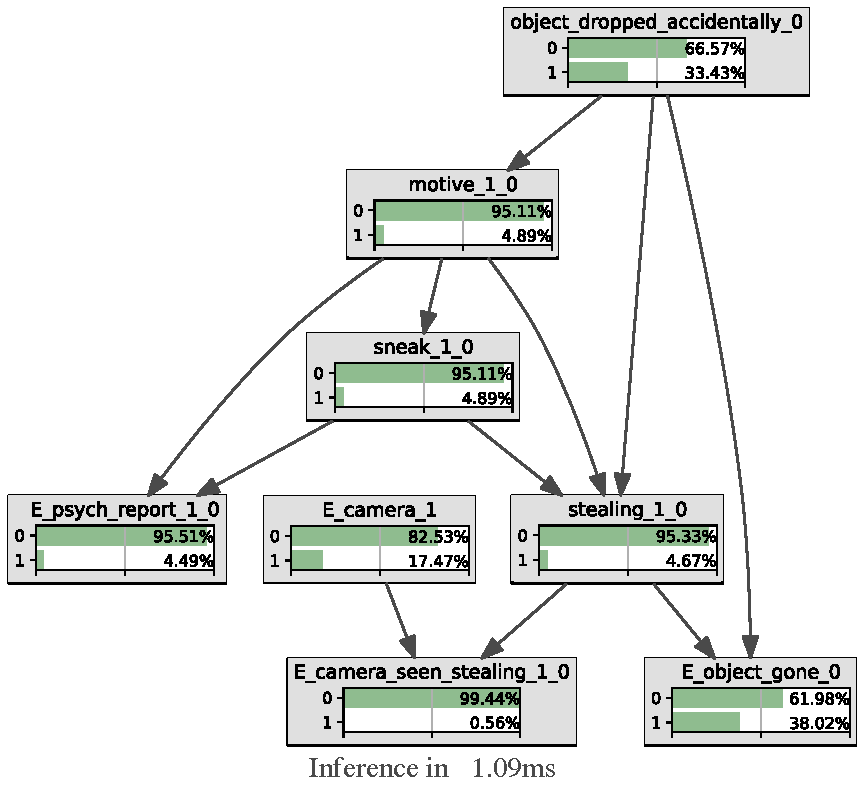
\includegraphics[width=\linewidth]{GroteMarktPrivate/bnImage/BNIMAGEGroteMarktPrivate500.pdf}
\caption{The final network (500 runs)}
\end{subfigure}
\begin{subfigure}{0.45\textwidth}
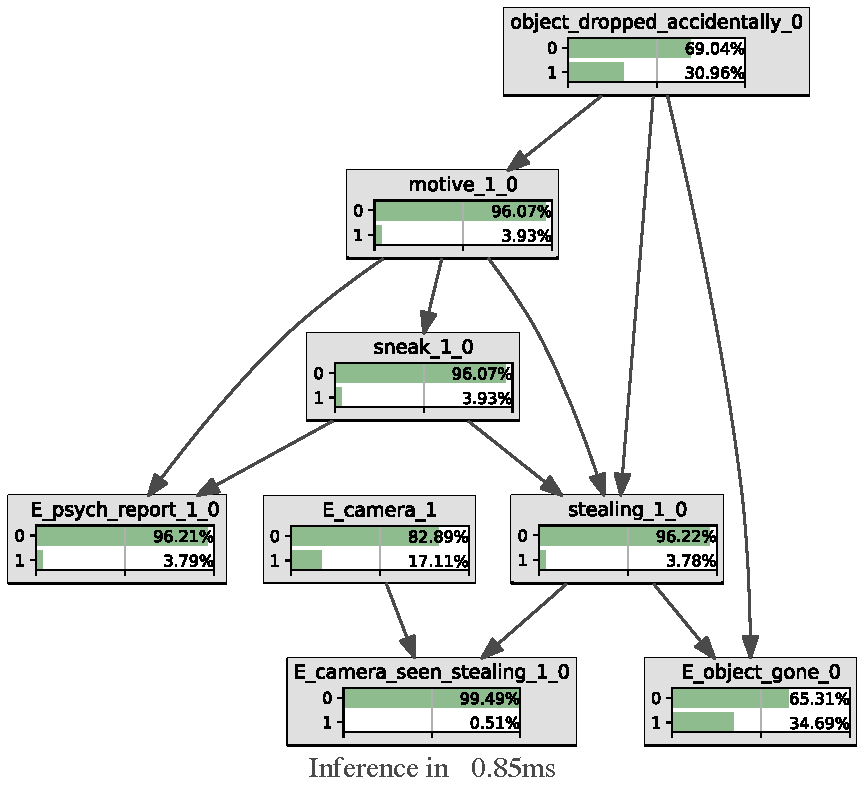
\includegraphics[width=\linewidth]{GroteMarktPrivate/bnImage/BNIMAGEGroteMarktPrivate750.pdf}
\caption{The final network (750 runs)}
\end{subfigure}
\begin{subfigure}{0.45\textwidth}
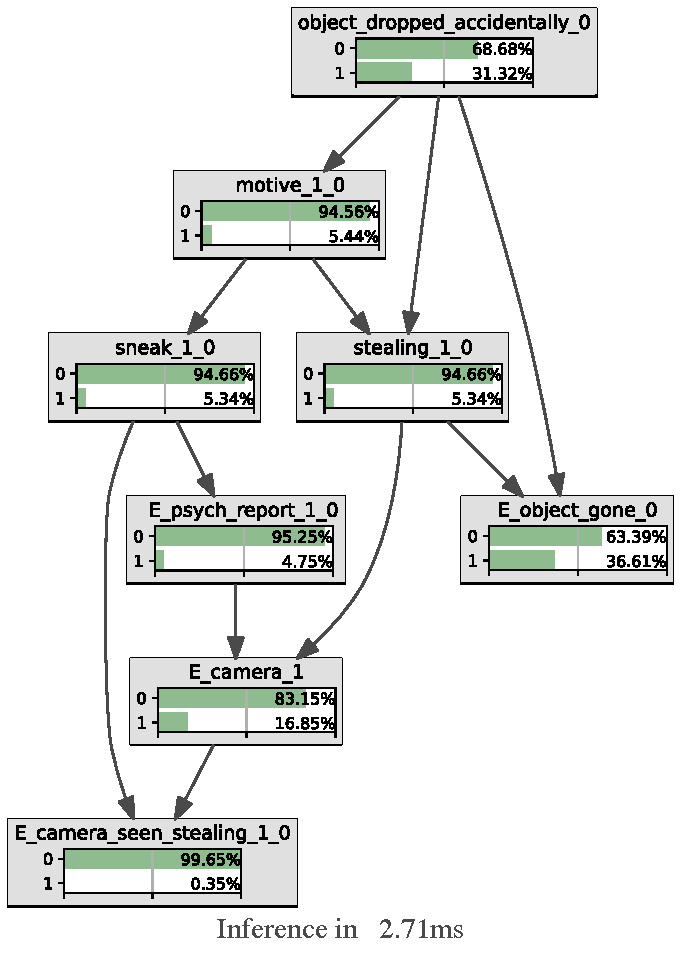
\includegraphics[width=\linewidth]{GroteMarktPrivate/bnImage/BNIMAGEGroteMarktPrivate1000.pdf}
\caption{The final network (1000 runs)}
\end{subfigure}
\caption{All final networks}
\label{bullet}
\end{center}
\end{figure}

For each of these networks, we set the possible evidence states as outlined in the case study. This means that, for every possible combination of evidence, we find the posterior probability of every output node. This results in a joint probability distribution over all three possible outputs. These are found for all evidence states, for every number of runs~\footnote{Excluding 1, as this did not result in a network}, in Tables~\ref{T50} --~\ref{T1000}. We can already see here that there are networks that produce inconsistent results. For example, see the evidence state of (1, 0, 0, 1) in Table~\ref{T50}. In this state, we find that P(neither) $= -0.26$. This shows that this network cannot represent accurately the mutual exclusive and exhaustive relationship of the three output nodes. As the dataset from which the networks are built increases in size, these inconsistencies decrease.

\input{tableAutomatic.tex}

Now that we have the posterior probabilities for all outputs for all evidence states, we present the accuracy of the network, by comparing the posterior output of every BN to the `ground truth' frequency-output of the simulation. The accuracy per output node, for every state of evidence, is presented in Table~\ref{eye}. Overall, the networks have an accuracy of 0.88. Networks that are created from a larger dataset, have higher accuracies than networks generated from smaller accuracies.

\begin{table}[htbp]
\footnotesize
\centering
\begin{tabular}{|l|c|c|c|c|c|c|c|c|c|c|c|c|c|c|}
\hline
	runs				&	\multicolumn{2}{|c|}{50}  &	\multicolumn{2}{|c|}{100}	&	\multicolumn{2}{|c|}{300} &	\multicolumn{2}{|c|}{500}	&	\multicolumn{2}{|c|}{750}&	\multicolumn{2}{|c|}{1000}	 & 	av	\\
\hline
	evidence						&	S	&	D	&	S	&	D	&	S	&	D	&	S	&	D	&	S	&	D	&	S	&	D	&		\\
\hline
(0, 	0, 	0, 	1) 				& 	0.99 & 1.00&	1.00 & 1.00	&	0.99 & 0.99	& 	0.98 & 0.98	& 	0.99 & 0.99	& 	0.99 & 0.99 & 0.99	\\
(0, 	0, 	0, 	0) 				& 	1.00 & 1.00&	1.00 & 1.00	&	1.00 & 1.00	& 	1.00 & 1.00	& 	1.00 & 1.00	& 	1.00 & 1.00& 1.00	\\
(0, 	1, 	0, 	1) 				& 	0.98 & 0.98&	0.99 & 0.99	&	0.99 & 1.00	& 	0.98 & 0.98	& 	0.99 & 0.99	& 	0.92 & 0.92& 0.98	\\
(1, 	0, 	0, 	1) 				& 	0.47 & 0.21&	0.66 & 0.64	&	0.98 & 0.97	& 	0.95 & 0.95	& 	0.94 & 0.94	& 	0.96 & 0.96& 0.80	\\
(0, 	1, 	0, 	0) 				& 	0.89 & 0.85&	1.00 & 1.00	&	1.00 & 1.00	& 	1.00 & 1.00	& 	1.00 & 1.00	& 	1.00 & 1.00& 0.98	\\
(1, 	1, 	0, 	1) 				& 	0.97 & 0.86&	0.20 & 0.20	&	0.75 & 0.75	& 	0.95 & 0.95	& 	0.94 & 0.94	& 	0.94 & 0.94& 0.78	\\
(1, 	1, 	1, 	1) 				& 	0.96 & 0.87&	0.95 & 0.98	&	0.95 & 0.96	& 	0.93 & 0.93	& 	0.95 & 0.95	& 	0.96 & 0.96& 0.95	\\
(1, 	0, 	0, 	0) 				& 	0.78 & 0.79&	0.56 & 0.80	&	0.88 & 0.96	& 	0.62 & 0.89	& 	0.93 & 0.98	& 	0.75 & 0.92& 0.82	\\
(0, 	1, 	1, 	1) 				& 	0.88 & 0.73&	0.53 & 0.42	&	0.87 & 0.84	& 	0.03 & 0.03	& 	0.71 & 0.70	& 	0.96 & 0.96& 0.64	\\
\hline
total    						& 	0.88 &  0.81 & 0.766 &  0.781 &    0.934 &  0.941   &     0.827 &  0.857 &    0.939 &  0.943 &     0.942 &  0.961   & 0.88 \\
\hline
\end{tabular}
\caption{Accuracy per state}
\label{eye}
\end{table}

In Figure~\ref{girl}, we average over all possible evidence states and show the average accuracy of the output nodes `stealing\_1\_0' and `object\_dropped\_accidentally\_0', per number of runs, as well as the accuracy of the preference ordering. We also present the frequency of the states in the grounding simulation (Figure~\ref{boy}).

\begin{figure}[htbp]
\begin{center}
\begin{subfigure}{0.49\textwidth}
\includegraphics[width=\linewidth]{../../FINALACCURACY.pdf}
\caption{Accuracy of network based on the number of training runs}
\label{girl}
\end{subfigure}
\begin{subfigure}{0.49\textwidth}
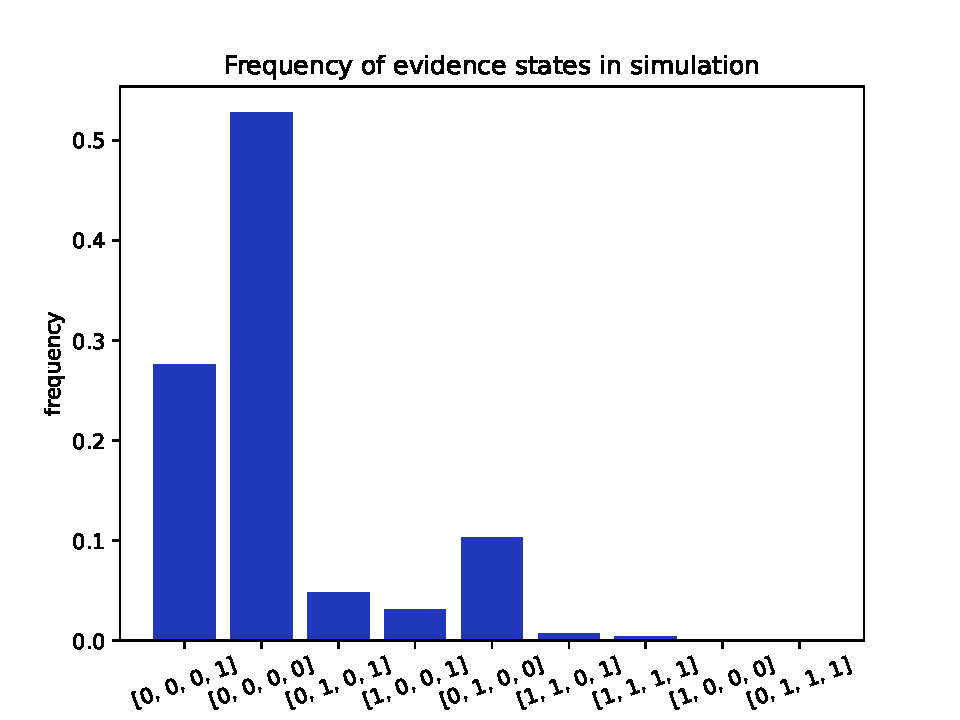
\includegraphics[width=\linewidth]{GroteMarktPrivate/plots/freqStates.pdf}
\caption{Frequency of network based on the number of training runs}
\label{boy}
\end{subfigure}
\end{center}
\end{figure}




\newpage



\section{Discussion}
The aim of this discussion section is to critically examine both Bayesian Networks and the proposed method for evaluating the BNs over all evidence states. In this section, we discuss the results and try to generalise this method to BNs that are made without the aid of simulations, so the networks from criminal cases that we are likely to encounter in the literature. We discuss whether this method is plausible in real life. Finally, we discuss the use of simulations for investigating Bayesian Networks and for modelling criminal cases.

\begin{itemize}
\item First, we consider the limitations that we find when applying the method to our case study, as outlined in the previous two sections. 
\item Second, we move one step away from this idealised situation, and attempt to construct a Bayesian Network for the situation in the case study manually, hence, not using the automatic BN constructor algorithm, but instead relying on causal knowledge and subjective probability estimates by the modeller. The purpose of this is to evaluate if a modeller can construct a network of similar accuracy to the automatically constructed networks. 
\item Third, we discuss the use of this method of evaluation for investigating existing Bayesian Networks. We investigate whether we can evaluate modelling primitives or idioms for Bayesian Networks, such as those in \citep{deZoete2019}. Additionally, we investigate whether this method of evaluation would be suitable for a Bayesian Network of a criminal case, as modelled in \citep{vanLeeuwen2019}. This leads to a discussion of the problem of combinatorial explosion in the number of evidence nodes.
\item Fourth, we discuss the implications of the findings in the discussion.
\item Finally, we discuss the use of simulations as a modelling primitive with a focus on operationalisation of nodes.

\end{itemize}


\subsection{Evaluating BNs over all possible evidence states using the simulation}

With this method, we can evaluate the accuracy of the BN of the criminal scenarios that we have automatically generated. In the evaluation, we find that the BNs predict posterior probabilities for the outputs that correspond to the limiting frequencies of events in the simulation. We can see this in the overall accuracy of the networks, as presented in Table~\ref{eye}, which range between accuracies of 0.76 at the lowest, to 0.961 at the highest. This means that all BN reflects the frequencies in the simulation well, not just on one state of cumulative evidence, but on nearly all states of cumulative evidence. 

On some evidence states, the networks are consistently correct (average accuracy of state $\geq 0.98$, nearly regardless of the number of runs that the network was trained on. These are the states of (0, 0, 0, 1), (0, 0, 0, 0), (0, 1, 0, 0), (0, 1, 0, 1). These are also the states that occur most frequently (see Figure~\ref{boy}).

For the other evidence states, increasing the number of runs (the data) available to the network, increases the performance. If we look at the frequency diagram in Figure~\ref{boy}, this is sensible: as we increase the data available to the network, the performance of the network will increase.


This method also allows us to see when the BN is assigning probability values to mutually exclusive nodes that violate probabilistic constraints. The joint probability over all three scenarios can never be greater than 1, which means that none of the probability values of `stealing\_1\_0', `object\_dropped\_accidentally\_0', and neither, can be smaller than 0. However, in Tables~\ref{T50},~\ref{T100},~\ref{T300},~\ref{T750}, we find that P(`neither') can be smaller than 0 for some evidence state.  This shows that the mutually exclusive relation between stealing and dropping is not learned correctly in the network. This improves when the K2 algorithm has access to more data.


Therefore, we find that this method of evaluating a BN over all states of cumulative evidence can distinguish between better and worse BNs: the best network is the network based on 1000 runs, which has an overall accuracy of 0.95. The method also shows for which evidence state the network performs badly, although it does not the modeller insight in how the network should then be changed to improve it. 

However, there are some limitations. There is a high variability between runs: if we were to run this experiment twice, we would find a different network structure for all networks, as well as different probabilities predicted. However, the average trend in increasing accuracy with a higher number of states remains. Additionally, finding the proper limiting frequency for the simulation is difficult. We ran the simulation 10,000 times, however, the simulation did not allow a state that should have been possible. The state where the thief-agent was seen by cameras, the psychological report states that it is guilty, but it was not seen stealing, and the object was not gone (1, 1, 0, 0). In the simulation, this state should be possible: the thief must have a motive, but fail to steal from the victim, which should be possible but very unlikely in the simulation. However, the combination of (psychological report = 1, camera = 1), happens only 118 times. Out of those 118 runs, in the simulation it is always the case that the object is gone. However, in theory, it should be possible that the agent has a psychological report that indicates he will steal, that he's seen on camera, yet does not steal. Increasing the number of runs from 10,000 to 100,000 might result in this state being reached.



\subsection{Can a modeller do this?}
We have shown that we can generate Bayesian Networks and evaluate them over all possible evidences states automatically, if we use the data as generated in training runs by the simulation. However, the real problem is, if a modeller could actually attempt to create a BN by hand without access to the underlying frequencies from the simulation. If we have a manually-crafted BN, but we also have the underlying true joint probability distribution over all variables in the simulation, we can test if this method of evaluation can show problems with a manually constructed Bayesian Network. 

In this section, we manually create a Bayesian Network for the scenarios as given in the case study: a (potential) robbery at the Grote Markt. This was done by imagining how a modeller would manually create a BN if they only had access to the simulation. Instead of looking at the source code of the simulation, the modeller would have access to the visual of the simulation, and would be able to run the simulation multiple times. The used reporters are given to the modeller, they are the same reporters that are used in the case study. However, the modeller should construct the structure of the BN, and fill the CPTs of the nodes, using their subjective estimation of causality and frequency of events in simulation. This was done to discuss the influence that the real lack of data, time and control would have on a modeller in a real criminal case.  





\subsubsection{Constructing the Manual Network}

We followed the construction methods as outlined in \citep{vlek2016} and \citep{vanLeeuwen2019}. We considered the three different scenarios: 1) the object was stolen, 2) the object was dropped, 3) neither happened. Since we use the same nodes as in the simulation, we do not have a separate node for scenario 3, or a constraint node. Scenario 3 is represented by both other scenarios having low probabilities.
 
 \begin{enumerate} 
 
\item Structure within scenarios: The hypothesis nodes of the two scenarios represented explicitly in the networks are: 1: [motive\_1\_0, sneak\_1\_0, stealing\_1\_0], and 2: [object\_dropped\_accidentally\_0]. Within every scenario, we are creating temporal arcs between the hypothesis nodes. For scenario 2, this is easy, since it consists of only 1 node and we do not need to add arcs. For scenario 1, we observe in the simulation that a motive comes before sneaking, which comes before stealing. Hence we identify [motive $\rightarrow$ sneak $\rightarrow$ stealing] as the structure of scenario 1.

\item Structure between scenarios. We need to know which scenario is the parent of the other scenario. Using the causality as described in Section 4.4, we place `object\_dropped\_accidentally\_0' before the first node of scenario 1. This results in the BN \[object\_dropped\_accidentally\_0 \rightarrow motive\_1\_0 \rightarrow sneak\_1\_0 \rightarrow stealing\_1\_0\]

\item Evidence nodes. For each node, we consider causality. `E\_psych\_report\_1\_0' relates to `motive\_1\_0' only, `E\_object\_gone\_0' to both `stealing\_1\_0' and `object\_dropped\_accidentally\_0', then `E\_camera\_seen\_stealing\_1\_0' only directed to `stealing\_1\_0', with as parent `E\_camera\_1'. 

\item For each node, create subjectively estimated conditional probability tables. Even though we can find the exact probabilties, because we have them in the simulation, we are going to attempt to ignore these probabilities: the network was created without actively looking for reference to the probabilities or processes in the simulation. Additionally, the probabilities that could be entered into the CPTs were restricted, only certain values could be entered. The allowed probabilities are described in Table~\ref{atp}


\begin{table}[htbp]
\begin{center}
\begin{tabular}{|l|l|}
\hline
Probability value & Explanation \\
\hline
0 & Never possible under any circumstance \\
0.01 & Very unlikely, but possible \\
0.25 & Could happen, but improbable \\
0.5 & Either state is equally plausible\\
0.75 & Is likely to happen, but might not \\
0.99 & Very likely, but not certain \\
1 & Always, certain to occur \\
\hline
\end{tabular}
\end{center}
\caption{Allowed probabilities and their meaning in natural language}
\label{atp}
\end{table}

The network is presented in Figure~\ref{hebben}. The CPTs for the nodes are presented in the Appendix 8.1.
 
 \end{enumerate}
 
 
\begin{figure}[htbp]
\begin{center}
\includegraphics[width=0.7\linewidth]{images/manualNetwork.pdf}
\caption{Manual network}
\label{hebben}
\end{center}
\end{figure}


\subsubsection{Evaluating the Manual Network}

\begin{enumerate}
\item \textbf{Run} We run the simulation 10,000 times to collect the ground truth.
\item \textbf{BN} We test the manual network (Figure~\ref{hebben}).
\item \textbf{Selection} The evidence nodes of the network are the 4 (binary) nodes marked with an `E', which are [E\_camera\_1, E\_camera\_seen\_stealing\_1\_0, E\_object\_gone\_0, E\_psych\_report\_1\_0]. The output nodes are [`object\_dropped\_accidentally\_0', `stealing\_1\_0'].
\item \textbf{Order} We order the evidence nodes in the same order in which we test the automated networks [E\_psych\_report\_1\_0, E\_camera\_1,  E\_camera\_seen\_stealing\_1\_0, E\_object\_gone\_0~].
\item \textbf{Collect} There are $2^4 = 16$ evidence states in total.
\item \textbf{Subset} See Table~\ref{wake}
\item \textbf{Frequencies} See Table~\ref{heretic}.
\item \textbf{Posteriors} For every evidence state, we use the BN in Figure~\ref{hebben} as model. In the BN, we turn the evidence nodes to the value specified by their evidence state. We used the LazyPropagation inference engine in PyAgrum to calculate the posteriors of the outcomes in the BN, given the evidence state as input. The posteriors are collected in Table~\ref{wife}. 
\item \textbf{Accuracy Evidence State} The posteriors of the outcome nodes in the network are compared to frequency of those outcomes in the ground truth. The accuracy of the BN per evidence state is presented in Table~\ref{now}.
\item \textbf{Accuracy Total} We find that, in total, the accuracy for this manual network is 0.71 for the `stealing\_1\_0' node, and~0.81 for the `object\_dropped\_accidentally\_0' node, with an average accuracy of~0.76. 
\end{enumerate}

These accuracy scores mean that the manual network performs slightly worse than the average of the automatically constructed networks (0.88). We see that there are only two cases where the manual network predicts the wrong output: the evidence set (0, 0, 0, 1), and the evidence set (1, 1, 0, 1). We treat these in turn.

\begin{itemize}
\item (0, 0, 0, 1): if the object is gone, but there is no other evidence, the manual network predicts that the object is stolen (0.55) rather than dropped (0.45), so about equally likely. The prior probability of the `object\_dropped\_accidentally\_0' node is 0.01, which corresponds to a subjective estimate of `Very unlikely, but possible'. Apparently, we have underestimated the amount of times that an object was dropped, rather than stolen (given that all other evidence is 0): in the simulation, if there is no further evidence, it is much more probable that the object was dropped than stolen.
\item (1, 1, 0, 1): if the psychological report is true, the potential thief was seen on camera, but was not seen stealing, and the object is gone. In this case, the network should predict that the agent has stolen. However, instead, the manual network breaks (hence, the probability assignments of -1). This combination of evidence is impossible in the network, but it should be allowed, as it is a possible state in the simulation.
\end{itemize}



\begin{table}
\centering
\small
\begin{tabular}{|l|c|c|c|}
\hline
evidence & H1 & H2 & H3 \\
\hline
(0, 0, 0, 1)&P(steal) (0.55) & P(dropped) (0.45) & P(neither) (0.00) \\
(0, 0, 0, 0)&P(neither) (1.00) & P(steal) (0.00) & P(dropped) (0.00) \\
(0, 1, 0, 1)&P(dropped) (1.00) & P(steal) (0.00) & P(neither) (0.00) \\
(1, 0, 0, 1)&P(steal) (1.00) & P(dropped) (0.00) & P(neither) (0.00) \\
(0, 1, 0, 0)&P(neither) (1.00) & P(steal) (0.00) & P(dropped) (0.00) \\
(1, 1, 0, 1)&P(neither) (3.00) & P(steal) (-1.00) & P(dropped) (-1.00) \\
(1, 1, 1, 1)&P(steal) (1.00) & P(dropped) (0.00) & P(neither) (0.00) \\
(1, 0, 0, 0)&P(neither) (1.00) & P(steal) (0.00) & P(dropped) (0.00) \\
(0, 1, 1, 1)&P(steal) (1.00) & P(dropped) (0.01) & P(neither) (-0.01) \\
\hline
\end{tabular}
\caption{ Preference ordering with numbers for manual network}
\label{wife}
\end{table}%


\begin{table}[htbp]
\begin{center}
\begin{tabular}{|l|c|c|}
\hline
evidence & steal & dropped  \\
\hline
(0, 0, 0, 1) & 0.46 & 0.46  \\
(0, 0, 0, 0) & 1.00 & 1.00 \\
(0, 1, 0, 1) & 0.99 & 0.99 \\
(1, 0, 0, 1) & 0.93 & 0.93 \\
(0, 1, 0, 0) & 1.00 & 1.00 \\
(1, 1, 0, 1) & -0.93 & -0.07\\
(1, 1, 1, 1) & 0.95 & 0.95\\
(1, 0, 0, 0) & 1.00 & 1.00 \\
(0, 1, 1, 1) & 1.00 & 0.99\\
\hline
total & 0.711 &  0.806  \\
\hline
\end{tabular}
\end{center}
\caption{Accuracy per evidence state per output node}
\label{now}
\end{table}

 \subsubsection{Discussing the Manual Network}
 
We find that the manual network performs well, with a 0.76 accuracy, which is only slightly worse than the automated networks. It is not the case that the accuracy per evidence state is low, instead, the performance is very accurate over most evidence states, with only two evidence states that cause the lower accuracy. This means that it would be possible to improve the network by focussing on the reason why, for these evidence states, the CPTs result in an incorrect prediction.Then, these CPTs can be changed, instead of trying to increase the performance of the network over all possible evidence states. Therefore, it seems possible that we can manually construct accurate BNs for crime cases, even with subjective probabilities. We can also use the method postulated in Section 3 as a way of evaluating the network to find where we might have over- or under-estimated probabilities in the CPTs, using the grounded frequencies generated from the simulation. Hence, a modeller might be able to construct a BN based on simple scenarios by hand. However, there are some limitations, both in how this network was created, as well as the evaluation method.

To address the main limitation first, ideally, this manual crafting of the BN should be done by someone who did not create the simulation. Involvement with the crafting of the simulation gives the modeller an unfair advantage compared to an `new' modeller in estimating probabilities and understanding the causal structures, as they know how the simulation works. Additionally, in real life, we do not have access to the source code of the universe either, but we still have to build a network. Hence, the manual network should not be constructed by the modeller who created the simulation. However, in this paper, only the modeller of the simulation was available to build the manual BN. This might have improved the accuracy of the manual network.

Additionally, there are three limitations regarding the evaluation method. First of all, we can only use the method to find an evidence state with a low accuracy, but we do not have a way of resolving the low accuracy. The method does not tell you which CPTs need to be changed in what way. Secondly, we can only use the accuracy measure when we have a grounding data, in this case from the simulation. In real life, modellers of criminal cases do not have this grounding data. Finally, we find a problem in the selection of the possible states. In the simulation, some evidence states are not allowed, they have a frequency of 0. For most of these states, the manual network results in an error if these states are entered, as it should. This is where Bayesian Networks can guide the modeller in correctly reasoning about evidence. However, the manual network allows one state of evidence that is not allowed in the simulation, which is the state of (1, 1, 0, 0). This is the state where the `thief' has a psychological report stating that they could steal, they were seen on camera, but they were not seen stealing, and, most crucially, the object is not gone. This is a case where human intuition and what should happen, clashes with the frequencies of what actually happens in the simulation.


\subsection{Evaluating BNs over all possible evidence states in real life}

In this section we evaluate two Bayesian Networks with the method outlined in Section 3.4. 

 \subsubsection{de Zoete 2019}
 
The first is a network by de Zoete et all, about child abuse. This is from a paper about probabilistic paradoxes in legal reasoning \citep{deZoete2019}. The paper considers a case where we want to know if a child is abused. We have a certain behaviour that is associated with abuse, but some study shows that this behaviour occurs equally frequently in children who are not abused. Only when the behaviour $EB$ occurs together with an additional characteristic $AC$, there's a strong probability of abuse. It has been proposed that the combination of two evidence pieces is difficult to model - however, de Zoete at all find a way to model it, using the BN presented in Figure~\ref{pity}. In this network, they divide the potential children into three groups: 1) a child who is abused, who must exhibit both the behaviour and the additional characteristic, 2) a child who is not abused, who has the behaviour but can never have the additional characteristic, and 3) a child who is not abused, who does not have the behaviour, and also does not have the additional characteristic.
 

 \begin{figure}[htbp]
\begin{center}
\includegraphics[width=\linewidth]{images/abusedNetworkImage.pdf}
\caption{Abuse Network, replicated from \citep{deZoete2019}}
\label{pity}
\end{center}
\end{figure}

In the paper, a table is presented with the possible outcomes of the network to show that the network models the apparent paradox correctly. Turning either one of the nodes $EB$ or $AC$ on (and leaving the other unspecified) does not affect the probability of the child being abused. This was 0.4, and remains 0.4. However, if we set both $EB$ and $AC$ to `true', results in a posterior probability of abuse of 1, as expected.

Now, we apply the method of evaluating the network over all possible evidence states. We did not create a simulation for this, hence we cannot apply the full method.

\begin{enumerate}
\item \textbf{Run} We cannot run a simulation.
\item \textbf{BN} We test the manual network (Figure~\ref{pity}).
\item \textbf{Selection} The evidence nodes of the network are the 2 binary nodes $EB$ and $AC$. The output node is the ternary node $Group$.
\item \textbf{Order} We order the nodes based on the order implied in the text: we care about the exhibited behaviour ($EB$) first, then look at the additional characteristic $AC$.
\item \textbf{Collect} There are $2^2 = 4$ evidence states in total.
\item \textbf{Subset} All evidence states are possible.
\item \textbf{Frequencies} We cannot calculate frequencies.
\item \textbf{Posteriors} For every evidence state, we use the BN in Figure~\ref{pity}. In the BN, we turn the evidence nodes to the value specified by their evidence state. We used the LazyPropagation inference engine in PyAgrum to calculate the posteriors of the outcomes in the BN, given the evidence state as input. The posteriors are collected in Table~\ref{ipad}. 
\item \textbf{Accuracy Evidence State, Total} We cannot calculate an accuracy.
\end{enumerate}

Even though we have not simulated this scenario and hence have no baseline, we can still evaluate the posterior of the network based on our subjective expectations of how evidence should influence our reasoning. We see that the network performs as expected in 3 out of 4 cases. If we do not set any evidence, we just have the prior probability. Setting either one of the pieces of evidence to `false' reduces our belief in the posterior that the child has been abused (from 0.40 to 0.375 and from 0.40 to 0.25). This lines up with common sense: the evidence is negative, hence we reduce our belief in the posterior.

However, there we identify one strange case, presented in Figure~\ref{cowboy}, which is the case of both pieces of evidence being negative. So the child does not perform the behaviour and also does not have the additional characteristic. We would expect the probability that the child is abused to drop from 0.4 to something lower (perhaps not 0, but something lower). However, instead we find that the posterior of `abused' increases to 0.42. This does not seem like a conclusion that we want to draw. Unfortunately, it is unclear what is wrong with this network so we do not know why it produces a higher posterior belief in abuse if there is a total absence of evidence. We do not know how the CPTs should be changed in order to produce a network that conforms to our intuitions about the evidence. Hence, our method can only tell us that our network results in an unexpected outcome on some evidence state, yet does not tell us how to resolve this. 

 \begin{figure}[htbp]
\begin{center}
\includegraphics[]{../notebooks/FentonAbuse.pdf}
\caption{Posterior probability for abuse is higher than prior given that evidence is false}
\label{cowboy}
\end{center}
\end{figure}

\begin{table}
\centering
\small
\begin{tabular}{|l|c|c|c|}
\hline
Evidence  & P(abused) & p(nonAbusedBehaviour) & p(nonAbusednotBehaviour)  \\
\hline
no evidence set & 0.40 & 0.50 & 0.10 \\
$EB$ and $AC$ & 1.00 & 0 & 0 \\
$EB$ and $\neg AC$ & 0.375 & 0.625 & 0 \\
$\neg EB$ and $AC$ & 0.25 & 0 & 0.75 \\
$\neg EB$ and $\neg AC$ & 0.4286 & 0.4762 & 0.0952 \\
\hline
\end{tabular}
\caption{Posterior belief in either of the three hypotheses given evidence states}
\label{ipad}
\end{table}


\subsubsection{van Leeuwen 2019}
We applied the method for evaluating evidence on all evidence states to the network presented in \citet{vanLeeuwen2019}, shown in Figure~\ref{love}.  This network models a crime case where a suspect P murdered a tenant, then fled by car, and later called his parents to confess the crime, which is modelled as scenario 1 (scn1). In his own testimony, P states that he has amnesia and does not remember the day of the murder, and also that he was kidnapped, which is modelled as scenario 2 (scn2). The two scenarios are mutually exclusive and exhaustive.

\begin{figure}[htbp]
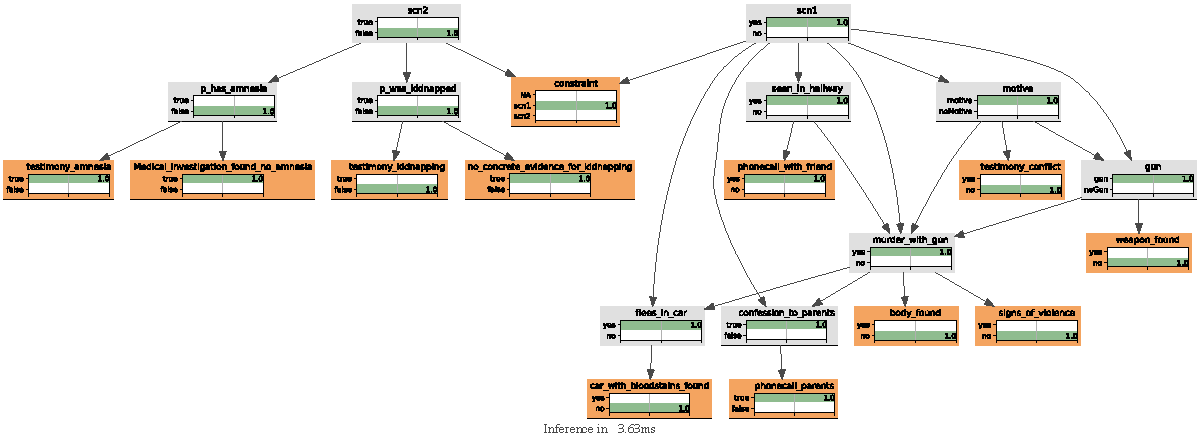
\includegraphics[width=\linewidth]{images/oldnetwork.pdf}
\caption{Example of subjective probability estimation resulting in a guilty verdict for insufficient evidence}
\label{love}
\end{figure}%


We did not create a simulation for modelling this scenario. It is not plausible for a network of this size to manually create the baseline by stating the expected posterior per outcome for every evidence state. Hence we have an ungrounded Bayesian Network. We cannot create a manual distribution over posteriors for a network of this size. The evaluation is as follows.

\begin{enumerate}
\item \textbf{Run} We cannot run a simulation.
\item \textbf{BN} We test a manually constructed network of the two alternative scenarios (Figure~\ref{love}).
\item \textbf{Selection} The evidence nodes of the network are the 11 binary nodes: `testimony\_amnesia' (TA), `Medical\_investigation\_found\_no\_amnesia' (MA), `testimony\_kidnapping' (TK), `no\_concrete\_evidence\_for\_kidnapping' (NK),
 `phonecall\_parents' (PP),  `car\_with\_bloodstains\_found' (CB), `body\_found' (BF), `signs\_of\_violence' (SV), `phonecall\_with\_friend'(PF), `testimony\_conflict' (TC), `weapon\_found' (WF). The output nodes are the nodes $scn1$, representing that suspect P is guilty, and $scn2$, representing that P is not guilty.
\item \textbf{Order} We order the nodes as we read them from left-to-right in the network, which is the order as presented in the \textbf{Selection} step.
\item \textbf{Collect} There are $2^{11} = 2048$ evidence states in total.
\item \textbf{Subset} Some evidence states are not possible. However, it is impossible to know which states are not possible, since we neither have a simulation that can only generate possible states, nor enough time to consider all possible combinations of evidence by hand.
\item \textbf{Frequencies} We cannot calculate frequencies.
\item \textbf{Posteriors} For every evidence state, we use the BN in Figure~\ref{love}. In the BN, we turn the evidence nodes to the value specified by their evidence state. We used the LazyPropagation inference engine in PyAgrum to calculate the posteriors of the outcomes in the BN, given the evidence state as input. Instead, A selection of interesting cases is presented in Table~\ref{cases}. Posteriors over all evidence states can be found in Table~\ref{look} in Appendix 8.2.
\item \textbf{Accuracy Evidence State, Total} We cannot calculate an accuracy.
\end{enumerate}

We find that we do not have to handle all 2048 evidence states. The network constrained some combinations of evidence states, in 56.25\% of evidence states, the combination of evidence was not allowed by virtue of the BN. In the remaining 896 evidence states, the evidence state was applied to the network and the posterior probability for scenario 1 and scenario 2 were calculated. In general, scenario 1 and scenario 2 are about equally preferred under the states of evidence, in 428 states, scenario 1 has a higher posterior probability. In 468 states, scenario 2 has a higher posterior. In 768 states of evidence, it is the case that either scenario 1 or scenario 2 is equal to 1, which means that we are fully convinced that that scenario is correct, which means that in half the cases, we fully believe scenario 1, and in the other half, we fully believe scenario 2.

\begin{table}[htbp]
\begin{center}
\begin{tabular}{|l|l|c|c|}
\hline
C & evidence & H1 & H2  \\
\hline
1 & TA, MA, TK, NK, CB, PP, BF, SV, PF, TC, WF & scn1 (1.00) & scn2 (0.00)\\
2 & TA, $\neg$MA, $\neg$TK, $\neg$NK, $\neg$CB, PP, $\neg$BF, $\neg$SV, PF, $\neg$TC, $\neg$WF & scn1 (1.00) & scn2 (0.00)\\
3 & TA, MA, TK, NK, CB, PP, $\neg$BF, $\neg$SV, PF, $\neg$TC, $\neg$WF & scn1 (0.00) & scn2 (1.00)\\
4 & TA, MA, TK, NK, CB, PP, BF, $\neg$SV, PF, $\neg$TC, $\neg$WF & scn1 (0.40) & scn2 (0.60)\\
5 & TA, $\neg$MA, TK, $\neg$NK, $\neg$CB, PP, BF, $\neg$SV, PF, TC, WF & scn1 (0.07) & scn2 (0.93)\\
6 & $\neg$TA, $\neg$MA, $\neg$TK, $\neg$NK, $\neg$CB, $\neg$PP, $\neg$BF, $\neg$SV, $\neg$PF, $\neg$TC, $\neg$WF & None & None\\

\hline
\end{tabular}
\end{center}
\caption{Interesting rows extracted from complete table}
\label{cases}
\end{table}


\begin{enumerate}
\item In case 1, we find that, if all evidence nodes are true, which is the situation as found in the court case, the network shows that scenario 1 is the case, and that the suspect is guilty, with a probability of 1. This is the expected output, and corresponds to the outcome of \citet{vanLeeuwen2019}.
\item In case 2, we find that there is no body, no signs of violence, no car with bloodstains, no evidence of existing conflict. The only evidence that the prosecution has, are two phone calls. The outcome of the network is that the suspect is guilty (P(scn1 = `yes') = 100\%). But the evidence that is entered into this network, would not reasonably support this conclusion. No reasonable arguer would argue that this state of evidence is sufficient for a guilty verdict.
\item In case 3, we fully believe scenario 2, so that the suspect is not guilty. However, all evidence that we have learned about scenario 2 shows that scenario 2 is not true: we have testimony for amnesia, but no medical record of it. We have testimony for kidnapping, but no concrete evidence for kidnapping. This should mean that our posterior belief in scenario 2 should decrease. We also have a little evidence on the side of scenario 1: two phone calls, and a car with bloodstains. This would not be enough for a conviction, but it should be enough that our belief in scenario 1 is not 0.
\item In case 4, we believe the same case as evidence state in case 3, but now we change our evidence. In case 3 we believe that we have not found a body. Now we add that we find the body, and we see that our belief in scenario 1 increases, from 0 to 0.40. This is a change of our belief in a reasonable direction given new evidence. The size of the belief-change, from 0 to 0.40, is difficult to assess without a realistic baseline.
\item In case 5, we find that the suspect says that he has amnesia and also that he was kidnapped, and this is supported by the other evidence. This adds support for scenario 2. However, we also find a lot of support for scenario 1: a body, a testimony of conflict, the phone calls, weapon found. Just not the car, and no signs of violence on the scene. Here, the modeller's subjective probability estimate is that, even though scenario 2 is supported by some evidence, scenario 1 has a higher probability than 0.07. Hence, the output does not line up with the modeller's expectation.
\item In case 6, we present a a special case: if all evidence nodes are false, the inference engine shows the result that the evidence is altogether incompatible. Since both scenarios are mutually exclusive and exhaustive, this result is sensible and shows that the BN can indeed structure our reasoning.
\end{enumerate}

Even without using a simulation, the evaluation method can be used to gain insight in whether the BN conforms to our expectations. We can identify cases where it seems to work correctly, such as case 1) and case 3). In case 1), the output conforms to the one datapoint that we have (given all evidence, the suspect is guilty), the BN makes the same decision as the court. In case 4), we find that the network, in this circumstance, responds sensibly to a change in evidence. However, in case 2), 3) and 5), we find the performance of the network not convincing. In case 2), there is insufficient evidence for scenario 1, yet the network chooses scenario 1. In case 3), there is insufficient evidence for scenario 2, yet the network chooses scenario 2. In case 5), there is support for both scenarios, but the posterior probability for scenario 1 seems (subjectively) too low. Furthermore, we now also know which states are deemed impossible (example: case 6). However, since we do not have a simulation or real-life test-cases, we do not have a way of `objectively' checking whether the network performs correctly or not, and to objectively identify combinations of evidence for which the network is performing badly. We can only do spot-checks and manually search through the output to see if we found anything interesting. Also, if we found a case for which the network performs incorrectly, it is also not clear what we should do with that: how should we change the probabilities in the CPT in order to increase `accuracy'?

It is possible to apply this method of evaluation to other networks based on criminal cases (given that they are produced in an open-access format), to non-systematically check the performance of these networks over all possible evidence valuations. In the networks as considered in the Anjum case study in \citet{vlek2016}, or the Simonshaven case in \citet{Fenton2019}, the evidence nodes are distinguished from the hypothesis nodes. Even without considering the temporality of evidence, we can set the cumulative evidence all at once. However, since we do not have simulations for grounding, or data for grounding, we cannot actually evaluate the networks based on `objective' measures. Manually considering all evidence sets will be even more problematic than before. Instead of 11 nodes, the Simonshaven network has 13 evidence nodes, and the Anjum network has 20 evidence nodes. If we assume that calculating 1 case will take around 0.0037 seconds (as calculated from 7.66 seconds for 2048 entries, this does not hold entirely because it also depends on the number of hypothesis nodes), producing all possible Simonshaven states and posteriors should take $2^{13} = 30$ seconds, which is still reasonable. The Anjum network would take 64 minutes. That is only considering the automatic calculation of the posteriors, and does not consider the time-complexity of creating a manual or automatic baseline. Additionally, some of the nodes in the Simonshaven are not binary nodes (`number of people in woods' has three possible states), resulting in a higher complexity as well. 




\subsection{Implications}

The discussion about the networks presented in this section suggest that there is a limited use for both ungrounded Bayesian Networks as well as for the evaluation method as outlined in the Method section.

In case of ~\citep{deZoete2019}, Figure~\ref{pity}, we are essentially investigating a method for creating a BN. This network is an implementation of a Bayesian Network idiom that is supposed to model the situation where either piece of evidence by itself is not enough to increase the posterior, yet both pieces of evidence together are convincing. This is an example of a BN idiom, like the other BN idioms that are presented in that same paper, as well as in \citet{Fenton2019}. Idioms generally have few nodes and the evidence states that are possible are clear, so we do not need a simulation to consider the possible states. In this case, we can use the method of evaluation, even without a grounding simulation, to discover the evidence states for which these idioms might behave unexpectedly.

However, this method of evaluating Bayesian Networks on all possible evidence states is not plausible for BNs that move away from abstracted, small idioms and attempt to model actual or fictional criminal cases. In the worst case, if we have $e$ evidence states, this means that we have $2^e$ possible evidence states. We would have to define a preference ordering or probability distribution on the output nodes in $2^e$ cases. This is plausible in a network with 4 evidence nodes, like the idiom-networks. However, networks that model criminal cases have more than 4 evidence nodes. This necessarily puts an upper bound on the level of granularity one can model in their network. If a network becomes more detailed in how evidence is represented, the higher the chance that considering all possible evidence states becomes impossible. A rough estimation shows that a 20-evidence-node network will take about an hour, but 20 pieces of evidence are not much in a complex case. Due to exponentiality, a network with 25 evidence nodes would result in 2.3 months of calculations.

If we take a different approach and attempt to create the BN from elicited, statistical information as found in the real world, we run into a different problem. Even though we might be able to find statistics about criminal behaviour, it is unclear to what extent those statistics would generalise towards probabilities in the network. For example, we might be able to estimate the proportion of Dutch people who own a gun. However, this information by itself hardly seems relevant when we look at the facts of the case as described in the case~\footnote{Case number: ECLI:NL:RBUTR:2004:AO3150}: the suspect was ex-military and might have killed someone with the same weapon before. Using a general statistic about gun-ownership in the Netherlands does not fit the case, hence, low generalisation: the statistics that we might use to `ground' the network might be irrelevant. Furthermore, we might not always be able to define which statistic is the most relevant. This is the fundamental `problem of the reference class' \citep{colyvan2001}.

Both these problems mean that we cannot know for which evidence states the network is accurate. Even if the manual, subjectively estimated networks have an accuracy of 0.76, as we have shown for the network in Figure~\ref{now}, we cannot be sure that this relatively high accuracy holds for a network that is as complex as the network in Figure~\ref{love}, or the networks in ~\citet{vlek2016} or ~\citet{Fenton2019}.
 We need to define many more cases of evidence than we are actually reasoning with. In the court cases, we are only considering evidence that we believe is true: we do not have to reason about what we would conclude if we had found the evidence in a different state. In BNs, we are implicitly defining the joint probability distribution over all possible evidence states: in the ~\citep{vanLeeuwen2019} network, all 2048 evidence states are defined implicitly, and for all these evidence states, the network must be correct. This is a very high bar to clear.


                                                                                                                                                                      
\subsection{Using Simulations as a modelling primitive}
Throughout this paper, we have used simulations as a modelling primitive, to ground our Bayesian Networks. In this section, I discuss some of the advantages and disadvantages of using simulations, compared to using Bayesian Networks by themselves.

\begin{itemize}
\item \textbf{Advantage: The Agent Metaphor}

Programming agents, and their interactions with their environment, make for a more intuitive modelling experience than attempting to find probabilities for events. We can ascribe intentions to agents and let them engage with the environment in a way that makes sense to us, by programming functional behaviour into them. This leads to an easier way of thinking about causality. If we were to model a murder, in a simulation, we have to explicitly represent how the murdering agent murdered the victim: if they used a weapon, did they have to grab it first? By locating the agents in an environment, it becomes easier to think about the preconditions that are necessary for behaviour and these can be programmed into the simulation in a sensible way.

\item \textbf{Advantage: Operationalisation}

In the simulation, you are forced to operationalise everything. We know exactly how we determine whether an event happened or not. Everything is legible. In Bayesian Networks, if is often unclear what a node name actually means, and what sort of event it represents. If we would create a BN that contained the node `sneak', what would that mean? In natural language, we would assume that this node means something like `some person sneaks up on another person'. However, how can we operationalise `sneaking'? If we create a method for determining `sneaking', will we know when this method wrongly says that someone is sneaking when they are not, or vice versa? The validity of the method in the simulation is unclear in real life. However, in simulation we do not have to consider this as a problem, because we have access to the complete state-space of the simulation.


\item \textbf{Disadvantage: Subjectivity}

The probabilities that we have to put in the simulation, either those that are randomly drawn from appropriate distributions for agent behaviour, or if they come from deterministic behavioural rules, or emerge from agent-environment interactions, are not `more objective' than those in a Bayesian Network. The rules that we choose to implement and the distributions that we draw from, are still reflections of the modeller's subjective estimates. In a sense, we have just moved subjectivity up a level compared to the BNs.


\item \textbf{Disadvantage: Complexity}

Simulations get too complex very quickly, since it is easy to implement all kinds of specific behaviours for the agents. Debugging a simulation is difficult especially one like the one in this paper, which does not have data from reality to compare it to.

\end{itemize}



\section{Conclusion}

\subsection{Summary}
We have shown that simulations can be used to ground Bayesian Networks and we created an evaluation method for them. Bayesian Networks can be created from the simulation automatically and these Bayesian Networks can be evaluated for accuracy over all evidence states systematically. We find that generally, the automated Bayesian Networks perform relatively well for each set of evidence, even when they do not have access to much data. Making more data available to the network-building algorithm improves performance. 

We also applied this method of evaluation to a network that was constructed by hand, which attempted to model the scenarios as modelled by the simulation. We found that the manual network performed worse, but not much worse, than the automated BNs. This means that, if a situation is simple enough and the modeller is able to subjectively estimate probabilities and represent causal relations, the final, manual network, can be accurate over most evidence states. We are able to know that this network performs well, due to the grounding frequencies of the simulation.

If we take the grounding frequencies, and the simulation, away, the method of evaluating over all possible sets of cumulative evidence does not hold up very well, especially in networks that instantiate actual crime cases, instead of networks that model idioms. There is a place for the evaluation method in systematically investigating the use of idioms, however, the method is unsuited for evaluating `real-life' networks, as we do not have grounding data, node definitions are unclear, and a time-complexity of $2^e$ that makes evaluating networks with $\geq 20$ nodes implausible.

 
\subsection{Future Research}

The simulation in this paper is not complex, and does not model reality in any realistic way. The purpose of this simulation was just to generate data, and did not need to reflect any specific facts about the world. However, agent-based modelling can be useful for investigating different aspects of Bayesian Networks, or reasoning with evidence more generally. Increasing the level of the simulation from level 0 to something that reflects reality is useful to investigate problems such as the Opportunity Prior as presented in \citet{Fenton2017}. 




\bibliographystyle{apalike}
\bibliography{masterThesisCitations}

\newpage
\section{Appendix}

This appendix contains:
\begin{itemize}
\item The CPT for the manually constructed network.
\item The probability distribution and preference ordering over outcomes for all possible evidence for the Jurix 2019 network.
\end{itemize}

\subsection{Network}
\input{cptManual.tex}
\subsection{Table}
\input{tableOrder.tex}

\end{document}  